\RequirePackage{lineno}
\documentclass{revtex4}
%\usepackage[pdftex]{graphicx}

\usepackage{amsmath,amsfonts,amssymb}
\usepackage[english]{babel}
\usepackage[latin1]{inputenc}
\usepackage[T1]{fontenc}
\usepackage{color}
\usepackage{float}
\usepackage{verbatim}
\usepackage{graphicx}
\usepackage{bm}
\usepackage{mathtools}
\usepackage{stmaryrd}
\usepackage{anyfontsize}

\usepackage[font={small}]{caption}
\usepackage{subcaption}
\captionsetup{compatibility=false}
% \usepackage{xr}
% \externaldocument[extfig-]{supp}
%\usepackage{epstopdf}
%\usepackage{array}
%\usepackage{tabularx}
%\usepackage{multirow}
\usepackage{color}
%\usepackage{multibox}
%\usepackage{rotating}
% \usepackage{lineno}

%\usepackage[left]{lineno}
%\usepackage[comma,sort&compress]{natbib}
%\usepackage{authblk}
%\usepackage{multicol}

% \usepackage{longtable}


\linespread{1.5}

% \usepackage[comma,sort&compress]{natbib}
% \bibpunct{[}{]}{,}{a}{}{;}

\renewcommand{\thesection}{\arabic{section}}


\bibliographystyle{prsb}

% \usepackage{bibunits}

\newcommand{\beginsupplement}{%
        \clearpage
        \setcounter{table}{0}
        \renewcommand{\thetable}{S\arabic{table}}%
        \setcounter{figure}{0}
        \renewcommand{\thefigure}{S\arabic{figure}}%
     }

% \pagewiselinenumbers
\linenumbers
% \setlength\linenumbersep{3pt}

\begin{document}

% \Blindtext
%\title{Simple rules yield complex communities: deconstructed species interactions and the assembly of communities}
%\title{Community assembly and dynamics by the deconstruction of species interactions}
\title{Eco-evolutionary dynamics and collective dispersal: implications for salmon metapopulation robustness}
\author{
Justin D. Yeakel${}^{1,2,*}$, Jean P. Gibert${}^{1}$, Thilo Gross${}^3$, Peter A. H. Westley${}^{4}$, \& Jonathan W. Moore${}^{5}$ \\
${}^1$School of Natural Sciences, University of California, Merced, Merced CA, USA \\
${}^2$The Santa Fe Institute, Santa Fe NM, USA \\
${}^3$University of Bristol, Bristol, UK\\
${}^4$College of Fisheries and Ocean Sciences, University of Alaska, Fairbanks, Fairbanks AK, USA \\
${}^5$Earth${}_2$Oceans Research Group, Simon Fraser University, Burnaby BC, Canada \\
${}^*$To whom correspondence should be addressed: jdyeakel@gmail.com
}




\begin{abstract} %250 words
The spatial dispersal of individuals is known to play an important role in the dynamics of populations, and is central to metapopulation theory. At the same time, local adaptation to environmental conditions creates a geographic mosaic of evolutionary forces, where the combined drivers of selection and gene flow interact. Although the dispersal of individuals from donor to recipient populations provides connections within the metapopulation, promoting demographic and evolutionary rescue, it may also introduce maladapted individuals into habitats host to different environmental conditions, potentially lowering the fitness of the recipient population. Thus, dispersal plays a dual role in both promoting and inhibiting local adaptation. Here we explore a model of the eco-evolutionary dynamics between two populations connected by dispersal, where the productivity of each is defined by a trait complex that is subject to local selection. Although general in nature, our model is inspired by salmon metapopulations, where dispersal between populations is defined in terms of the straying rate, which has been shown to be density-dependent, and recently proposed to be shaped by social interactions consistent with collective movement. The results of our model reveal that increased straying between evolving populations leads to alternative stable states, which has large and nonlinear effects on two measures of metapopulation robustness: the portfolio effect and the time to recovery following an induced disturbance. We show that intermediate levels of straying result in large gains in robustness, and that increased habitat heterogeneity promotes robustness when straying rates are low, and erodes robustness when straying rates are high. Finally, we show that density-dependent straying promotes robustness, particularly when the aggregate biomass is low and straying is correspondingly high, which has important ramifications for the conservation of salmon metapopulations facing both natural and anthropogenic disturbances.
\end{abstract} 


\maketitle

\centerline{Salmon metapopulations, Straying, Dispersal, Eco-evolutionary dynamics, Alternative stable states}
\vspace{2mm}
\noindent {\bf Media Summary} 
Many migratory species, such as salmon, are remarkable in finding their way home. This homing has allowed fine-scale adaptations to the environments in which they evolve. But some individuals do not find their way home and instead stray to other locations, especially when there are fewer individuals to help with collective decision-making. With an eco-evolutionary model, we discovered that an intermediate and density-dependent straying rate allows linked populations to be robust to disturbance but maintain local adaptations.\\
% The rate at which individuals move within a metapopulation has large impacts on extinction risk. Among migratory species such as salmon, the rate of dispersal, also referred to as straying, may be density-dependent due to collective decision-making. We explore an eco-evolutionary model of two populations connected by dispersal, where the productivity of each is defined by a trait complex subject to local selection. We show that intermediate straying rates result in faster recovery times and more stable population dynamics, and that density-dependent straying tends to promote this robustness. These results have important ramifications for the conservation of salmon metapopulations facing both natural and anthropogenic disturbances.\\


\section{Introduction}

Intraspecific diversity can increase the resilience and stability of species or metapopulations. 
This diversity-stability linkage occurs when there are asynchronous population dynamics, where the changes in population size varies temporally across the metapopulation. 
This asynchrony will increase the potential for demographic rescue \citep{Brown:1977gk,Earn:2000fm} and also decrease the variability of processes that integrate across the metapopulation \citep{Anonymous:2015gf}. 
For example, different responses to climate variability within populations of a rare plant reduced fluctuations in abundance \citep{Abbott:2017hl}. 
This statistical buffer has traditionally been quantified as the Portfolio Effect (PE), which is the ratio of the population CV to the CV of the aggregated metapopulation \citep{Thibaut:2012km}. 
Strengthened portfolio effects are expected to increase the robustness of metapopulations to external disturbances, and by extension promote persistence \citep{Thibaut:2012km}.
In contrast, homogenization of populations leading to greater synchronization and weakened PE may be a harbinger of metapopulation collapse and extinction.


% Although dispersal and the consequent gene flow can influence the evolutionary dynamics of metapopulations, the interplay between selection, population dynamics, and persistence is not well understood.
Movement of individuals among local populations (i.e. dispersal) can have a large influence on metapopulation persistence \citep{MilnerGulland:2011vm}. 
Dispersal facilitates evolutionary rescue, whereby immigration of individuals with heritable adapative traits can rescue small populations from local extinction in the context of maladaptive environmental change \citep{Bell:2011ki,Carlson:2014is}.
% First, some level of straying is necessary to enable the rescue effect, whereby dispersal among populations can rescue small populations from local extinction (REFS). 
On the other hand, high rates of dispersal may synchronize populations and actually increase the risk of extinction of the entire metapopulation \citep{Earn:2000fm}. 
Dispersal will also influence the evolutionary dynamics of the metapopulation.
% though how the interplay between selection and population dynamics might impact persistence is less well understood. 
Although the dispersal of individuals into sites hosting other populations provides connections within the larger metapopulation, potentially promoting demographic and evolutionary rescue, it may also introduce maladapted individuals into habitats that are host to different environmental conditions, possibly lowering the mean fitness of the recipient population \citep{Muhlfeld:2014hs}. 
More broadly, dispersal can provide a mechanism by which phenotypes are sorted in space rather than time and facilitates the spread of maladaptive genes \citep{Lowe:2015ft}.
Dispersal in this case may lead to genetic homogenization that erodes the asynchrony underpinning portfolio effects and metapopulation persistence. 
% Thus, straying can influence the resilience and robustness of metapopulations through both ecological and evolutionary processes.
% Thus, the dual nature of straying as both promoter of connections among metapopulation demes and potential eroder of locally adapted gene complexes highlights the interplay between ecological dynamics of connected populations and the evolutionary dynamics of mixed trait distributions that respond to heterogeneous local conditions.


%Movement through space (link back to straying)
% Migratory populations that return to a breeding ground or natal stream to reproduce are linked to each other by some proportion of the population that permanently disperse, or stray into the `wrong' site. %; we might say that there is at least one \emph{Kevin} in every school or flock (figure \ref{fig:xkcd}).
There is growing appreciation that a combination of abiotic, biotic, and anthropogenic factors can control the rate of dispersal among populations \citep{H:2013fs,Keefer:2014gg,Bett:2017ha}.
Migratory populations that return to breeding sites for reproduction are linked to each other by some proportion of the population that permanently disperses into the `wrong' site. 
Recently, the role of social interactions and collective navigation has been hypothesized \citep[][this volume]{Berdahl:2015kv,Berdahl:2016dx,HardestyMoore:wg}.
The rate at which individuals disperse may be linked to errors made at an individual-level that are themselves diminished by migrating in groups and pooling individual choices \citep{Simons:2004jo,Berdahl:2015kv,Berdahl:2016dx}.
The potential influence of collective dispersal on the dynamics of individual populations and the metapopulation as a whole is a topic of considerable interest that has tangible conservation implications \citep{Brenner:2012gl,Johnson:2012fe,Fullerton:2011ii}.
% Whether and to what extent the ecological consequences of straying depend on the evolutionary dynamics that emerge from populations distributed across a selective gradient is unclear.
% How the assumed negative evolutionary effects of straying and subsequent gene flow is balanced by the positive effects of demographic rescue is the subject of this contribution.



%Eco-evolutionary dynamics in space
%% From geographic mosaic of coevolution to...
% That evolutionary forces of selection and gene flow play out heterogeneously across geographic mosaics is now a foundational concept in ecology and evolutionary biology \citep{Nuismer:1999ko,Thompson:2015hq,Nuismer:2000bb,Thompson:2005wf}.
% These mosaics are in part driven by environmental differences between habitats that alter the selective forces acting on different phenotypes \citep{Endler:1986tz}, and a principle underlying assumption is that there is gene flow such that individuals from different habitats mix over space \citep{Gomulkiewicz:2000bz,Thompson:2002hr,Nuismer:2003eh,Nuismer:2006be,Forde:2008kc,Guimaraes:2011hu,Gibert:2013hp}.
% Although the evolutionary outcomes of these spatial processes have been explored in depth (REFS), it is less well understood how selective mosaics and their consequent evolutionary forces impact population dynamics as they unpitchfork \citep{Hendry:2016un}.


%Motivation: straying
The eco-evolutionary impacts of dispersal likely have important implications for conservation and management in key taxa such as in migratory salmon.
While anadromous salmonid fishes (genera \emph{Oncorhynchus} and \emph{Salmo}) are renown for returning to their natal spawning habitats with high accuracy and precision after years at sea \citep{Quinn:2011tf,Jonsson:2011kg,Keefer:2014gg}, there are generally some individuals that `stray' (synonymously used hereafter to refer to dispersal) to non-natal sites to spawn \citep{Quinn:1993ge,Hendry:2004wf}.
Salmon may operate as metapopulations, where populations are genetically distinct but linked by some level of straying \citep{Schtickzelle:2007wb,Anderson:2014cx}.
Although extensive work has been done to document the extent of straying from donor populations into recipient populations \citep{Keefer:2014gg,Bett:2017ha}, only recently have the abiotic, biotic, and anthropogenic influences of straying behaviors been investigated systemically \citep{Keefer:2008bs,Westley:2015to,Bond:2016dz}.
Straying among salmon may be influenced by environmental factors such as water temperature, human activities such as hatchery practices, and population density as predicted by the collective navigation hypothesis \citep{Peterson:2014gy,Berdahl:2017uu}.
Straying can introduce new maladaptive genotypes into the recipient population, while the ensuing genetic homogenization could synchronize population dynamics and erode portfolio effects \citep{Moore:2010gs,Carlson:2011ce,Braun:2016ib}.
Thus, there is an opportunity and need to consider the eco-evolutionary consequences of straying for metapopulations in species of conservation and management concern such as salmon. 

% Asynchrony among salmon populations also increases the stability of fisheries that integrate across this diversity \citep{Schindler:2010he,Anonymous:2016jc}.
% However, these portfolio effects may be eroded if asynchrony is influenced by genetic diversity and this genetic diversity is lost. 
% Braun et al. \citep{Braun:2016ib} found that genetic differences among populations of Chinook salmon was correlated with the degree of asynchrony in population dynamics. 
% Artificial propagation of salmon by hatcheries and their strays may erode local genetic diversity, asynchrony among populations, and portfolio effects \citep{Carlson:2008hl,Moore:2010gs,Anonymous:2014ku}.  
%Coordinated mass migrations are one of the great wonders of the natural world, and the ability of individuals and groups to navigate across great distances have long fascinated naturalists \citep{MilnerGulland:2011vm}.

% Most recently the role of social interactions and collective navigation has been hypothesized \citep{Berdahl:2015kv,Berdahl:2016dx}.
% These strays can introduce new maladaptive genotypes into the recipient population.
% Straying amon salmon may be influenced by environmental factors such as water temperature, human activities such as hatchery practices, and population density as predicted by the collective migration hypothesis \citep{Peterson:2014gy}. 
% Thus, there is an opportunity to consider the eco-evolutionary consequences of straying for metapopulations in species of conservation and management concern such as salmon \citep{Carlson:2011ce}. 

% 
% \begin{figure}
%   \captionsetup{justification=raggedright,
% singlelinecheck=false
% }
% \centering
% 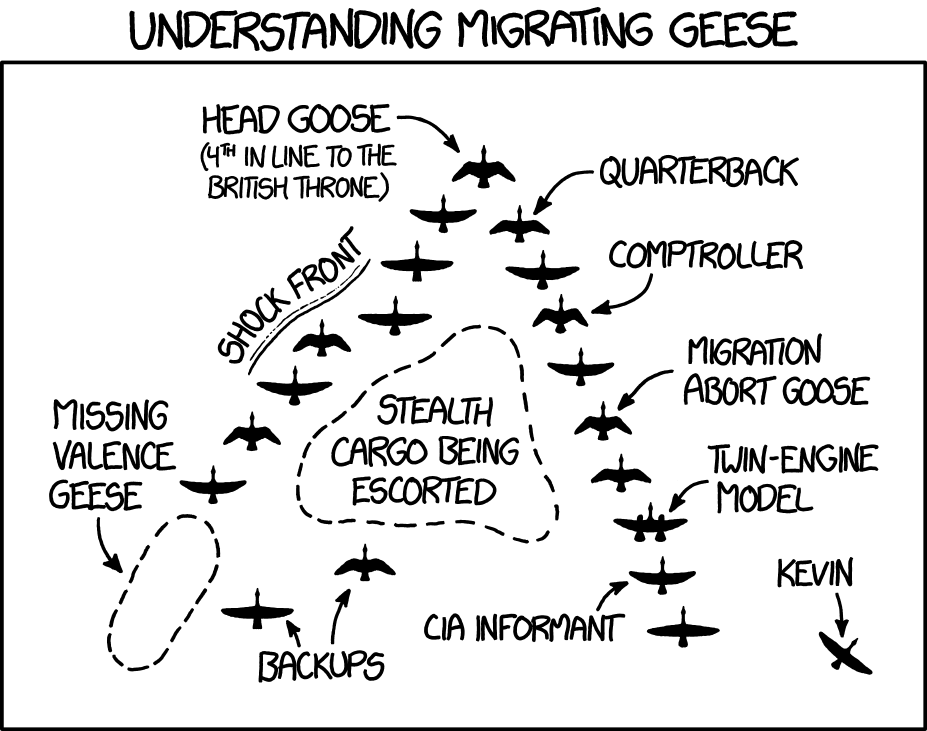
\includegraphics[width=0.4\textwidth]{figs2/fig_xkcd.png}
% \caption{
% \emph{Migrating Geese}, a comic from Randall Monroe's xkcd (https://xkcd.com/1729/). 
% A flock of geese travel in the direction of a shared destination, the lone stray named \emph{Kevin}.
% In this case, the rate of straying is $m=0.05$, which is not an uncommon rate for migrating populations of salmon \citep{Satterthwaite:2015ge}. 
% Reprinted under the Creative Commons Attribution-NonCommercial 2.5 License.
% } \label{fig:xkcd}
% \end{figure}

%Alternative stable state
Here we seek to explore how collective density-dependent straying influences the stability and robustness of metapopulations through ecological and evolutionary processes.
% the potentially detrimental evolutionary effects of straying (erosion of local adaptation) and subsequent gene flow is balanced by the positive effects of demographic rescue is the subject of this contribution.
% Here we ask the overarching question: how does collective behavior mediated dispersal and gene flow interact to influence the robustness of locally adapted populations?
To address this question we constructed a eco-evolutionary model of two populations occupying different sites that are linked by straying individuals, each with an associated trait distribution subject to natural selection determined by local conditions.
Specifically we compared (a) different rates of straying and (b) the influence of collective movement, across (c) increasing environmental heterogeneity, by assessing two measures of metapopulation robustness: the portfolio effect and the time required for a population(s) to recover following an induced disturbance. 
% This model enables us to explore the multiple and potentially opposing pathways by which straying influences metapopulation robustness such as the potentially detrimental erosion of local adaptation vs. the positive effects of demographic and evolutionary rescue.
This model enables us to explore the tradeoff between the potentially detrimental erosion of local adaptation vs. the positive effects of demographic and evolutionary rescue, both of which are facilitated by straying. %such as the potentially detrimental erosion of local adaptation vs. the positive effects of demographic and evolutionary rescue.

% [We show that taking straying into account leads to alternative stable states in population densities and trait values, which has consequences for maladaptation, intraspecific trait variability, and long-term sustainability of salmon metapopulations.]



\section{Model Description \& Analysis}

\noindent{\bf (a) Metapopulation framework}\\
\noindent We follow the basic framework provided by Ronce and Kirkpatrick \cite{Ronce:2001dp}, where dispersal connects two populations $N_i$ and $N_j$ that inhabit two distinct habitats, each with trait values $x_i$ and $x_j$ determining phenotype.
In our version of the model, there is an optimum trait value $\theta_i$ and $\theta_j$ associated with each habitat, where recruitment is maximized if the trait value of the local population equals the optimum, such that $x = \theta$.
Moreover, we assumed that $x_{i,j}$ are normally distributed with means $\mu_i$ and $\mu_j$ and have the same standard deviation $\sigma$.
As such, the recruitment rate $R_i[\mu_i(t),\theta_i]$ for both populations is determined by the mean trait value of the local population relative to optimal value at that site.
Trait means for each population are subject to selection, the strength of which is proportional to the difference between the trait mean and the local trait optimum at a given point in time \citep{simpson1953major,Lande:1976ga,Ronce:2001dp}.
% This framework mirrors the Ronce and Kirkpatrick model, except that selection is assumed to act on the rate of recruitment, rather than mortality.

%PW: Can we say anything about the effect of the recipient population size and that effect on evolutionary dynamics? Again, straying can be thought of as both from the donor or recipient population perspective.
The two populations occur in spatially separate sites that are close enough that a proportion of the population $m$ strays into the other site.
If there is no straying between these populations, then the mean trait evolves towards the optimal value for each site $\mu_i \rightarrow \theta_i$, and the recruitment rate for each population is maximized.
If there is straying between populations at rate $m$, then the traits in each respective location will be pulled away from the optimum, and recruitment rates will be lowered.
As $m \rightarrow 0.5$, the populations are perfectly mixed, effectively acting as a single panmictic population.


We used the discrete Ricker framework described by Shelton and Mangel \citep{Shelton:2011eq} as the basis for our two-site metapopulation model, with the added effect of the local population $N_i$ mixing with a proportion $m$ of individuals from a remote population $N_j$, and where there is no demographic overlap between generations.
In this sense, both populations serve simultaneously as donor and recipient populations.
Because total recruitment will be determined by both locals (with a mean trait value closer to the site optimum) and strays (with mean trait values farther from the local optimum), the recruitment of the aggregate is given by $R_i[\omega_i\mu_i(t) + (1-\omega_i)\mu_j(t),\theta_i]$ (Eq. \ref{eq:R}).
This mix of individuals is subject to identical compensatory effects, which is determined by the parameter $\beta$.
Taken together, the difference equation that determines changes in population size from time $t$ to $t+1$ is

\begin{align}
  &N_i(t+1) = R_i[\omega_i\mu_i(t) + (1-\omega_i)\mu_j(t),\theta_i] \\ \nonumber
  &\times \left((1-m)N_i + mN_j\right){\rm e}^{-\beta ((1-m)N_i(t) + m N_j(t))},
  \label{eq:N}
\end{align}

\noindent where

\begin{equation}
\omega_i=\frac{(1-m)N_i(t)}{(1-m) N_i(t) + m N_j(t)},
\end{equation} 
and the equation for $N_j$ mirrors that for $N_i$.

The recruitment of the population as a function of the mean trait value at time $t$ and the local trait optimum is

\begin{align}
  &R_i[\omega_i\mu_i(t) + (1-\omega_i)\mu_j(t),\theta_i] = \\ \nonumber
  &\int_{-\infty}^\infty r_{\rm max}\exp\left\{\frac{(x_i-\theta_i)^2}{2\tau^2}\right\} {\rm pr}(x_i,\omega_i\mu_i(t) + (1-\omega_i)\mu_j(t),\sigma^2) {\rm d}x_i +\tilde{P}_i\\ \nonumber
  &= \frac{r_{\rm max} \tau  }{\sqrt{\sigma ^2+\tau ^2}}\exp\left\{-\frac{(\theta_i-(\omega_i\mu_i(t) + (1-\omega_i)\mu_j(t)))^2}{2 \left(\sigma ^2+\tau ^2\right)}\right\} +\tilde{P}_i.
\end{align}

\noindent where the mismatch between the local trait mean $\mu_i(t)$ and the local optimum $\theta_i$ scales the recruitment rate for the population, and $\tilde{P}_i\sim {\rm Normal}(0,0.01)$ introduces a small amount of demographic error.
The parameter $\tau$ is the strength of selection, and controls the sensitivity of recruitment to changes in the mean trait value away from the optimum (the strength of selection increases with smaller values of $\tau$), which we set as $\tau=1$ here and throughout.
Because straying individuals are emigrating from a population with a mean trait value farther from the local optimum, their rate of recruitment is diminished.
Recent studies of wild sockeye salmon have indeed found that straying individuals have lower life-time fitness than individuals that do not stray, although it is unknown at what life-stage this selection occurs \citep{Peterson:2014gy}.
% The compensatory effects are then determined by the exponential, following the Ricker stock-recruitment relationship.
\\


% \noindent{\bf (b) Recruitment over a selective landscape}
Because individuals from the local population are mixed with individuals from the remote population via straying and subsequent reproduction, the resulting trait distribution is a complex mixture of trait distributions (see Supplemental Materials: Appendix I for the derivation, Fig. \ref{fig:PDF}).
We make two simplifying assumptions.
First, we approximate the distribution resulting from the mix of remote and local individuals prior to reproduction as a Gaussian, where $X_i=x_i$ with probability $g(x_i)$.
The expectation of the actual trait distribution as well as the Gaussian approximation are the same, such that ${\rm E}\{g(x_i)\} = \omega_i\mu_i + (1-\omega_i)\mu_j$, with weights corresponding to the proportion of the mixed population that are local individuals, $\omega_i$, and straying individuals, $1-\omega_i$.
Thus, strays can successfully reproduce and introduce their genotypes into the recipient population, which is supported by observations in wild populations \citep{Jasper:2013cc}.
Second, we assumed that changes in trait variance through time are minimal, such that $\sigma^2$ is constant over time, which is a common simplification in eco-evolutionary models of population dynamics \citep{Lande:1976ga,Ronce:2001dp,Schreiber:2011wx,Gilbert:2014ee,Gibert:2015kc}.
These simplifications are the same as those introduced by Ronce and Kirkpatrick, and were shown to have negligible impacts on dynamics \cite{Ronce:2001dp}.


% An increasing flow of incoming strays is generally expected to pull the mean trait value of the local population away from its optimum over time, which will decrease its rate of recruitment.
Following Lande \citep{Lande:1976ga}, and given our assumption of trait distribution normality, the mean trait value thus changes through time according to the difference equation

\begin{align}
  \label{eq:mu}
  \mu_i(t+1) &= \omega_i\mu_i(t) + (1-\omega_i)\mu_j(t) + h^2\sigma^2\frac{\partial}{\partial \mu^\prime}\ln\left(R_i[\mu^\prime,\theta_i] \right), \\ \nonumber
  &= \omega_i\mu_i(t) + (1-\omega_i)\mu_j(t) + h^2\sigma^2\left(\frac{\theta_i - \omega_i\mu_i - (1-\omega_i)\mu_j}{\sigma^2+\tau^2} \right),
\end{align}
given $\mu^\prime = \omega_i \mu_i(t)+ (1-\omega_i)\mu_j(t)$.
% This model formulation parallels that proposed by Ronce and Kirkpatrick \citep{Ronce:2001dp}, where habitat specialization evolves between two populations as a function of dispersal.
\\

\noindent {\bf (b) Density-dependent straying}
%Density-dependent m
\noindent We have so far assumed that the proportion of strays leaving and entering a population is constant, however there is mounting evidence that at least in some species (including salmon) straying is density-dependent, a signature of collective navigation \citep{Berdahl:2014bl,Berdahl:2017uu}.
Specifically, the rate at which individuals stray has been linked directly to a collective decision-making phenomenon, where greater numbers of individuals tend to decrease the rate at which individuals err, reducing the overall proportion of a population that strays.
According to Berdahl et al. \citep{Berdahl:2016dx}, given the probability that an individual strays is $m_0$, the proportion of the local population $N_i(t)$ that strays is

\begin{equation}
  m(t) = m_0\left(1- \frac{N_i(t)}{C+N_i(t)}\right),
  \label{eq:ddm}
\end{equation}

\noindent where $C$ is a half-saturation constant, and determines to what extent collective behavior, as a function of group size, diminishes straying.
If $C$ is small, relatively small groups of organisms `correct' for even high individual error rates, suppressing straying between sites.
In the context of our model, small values of $C$ indicate that the effects of collective behavior on modifying straying are strong.
As $C \rightarrow \infty$, groups of any size have no impact on straying, such that $m(t) \rightarrow m_0$, and the model reverts to that of constant straying.
When $C \ll \infty$ and the population density is high, $m(t) \rightarrow 0$, whereas if the population is small, individuals operate without regard to the collective, such that $m(t) \rightarrow m_0$, such that in all cases, $m(t) < m_0$.
% For realistic population densities, $m(t) < m_0$.\\
% We note that at the limit $C\rightarrow \infty$, the density-dependent straying rate becomes constant such that $m(t) \rightarrow m_0$, and this corresponds to the original formulation where $m=m_0$.


% \noindent {\bf (c) Habitat heterogeneity}
% \noindent Increasing differences in optimal trait values between sites ($\Delta\theta = \left|\theta_i - \theta_j\right|$) corresponds to greater regional differences in the conditions that favor alternative trait complexes, which can be interpreted as increased habitat heterogeneity.
% If both populations are isolated, natural selection will direct the mean trait values of both populations towards their respective optima, such that $\mu_i(t) \rightarrow \theta_i$ as $t\rightarrow\infty$.
% Habitat heterogeneity and the rate of straying are treated both independently, and as parameters that covary.
% In the latter instance, we examined a case where it is assumed that increased habitat heterogeneity correlates with lower straying rates, and vice versa (illustrated in figure \ref{fig:mthetarelation}).
% Two scenarios may lead to this correlation: 
% (\emph{i}) sites may be distributed over greater spatial distances, where habitat differences are assumed to be exaggerated and the likelihood of straying over greater distances is lower \citep{Candy:2000hu,JPE:JPE1383};
% (\emph{ii}) individuals may have behaviors promoting dispersal between habitats with structural or physiognomic similarities \citep{Peterson:2014gy}.
% In this case, the rate of straying would be greater between habitats with smaller differences in trait optima (lower $\Delta\theta$) and lesser between habitats with greater differences in trait optima (higher $\Delta\theta$).
% \\


\noindent {\bf (c) Measuring metapopulation robustness}
\noindent We evaluated metapopulation robustness by measuring the average-CV portfolio effect (PE) \citep{Anderson:2014cx,Schindler:2015gf} as well as the recovery time, which is the time required for the system to return to a steady-state following an induced disturbance to one or both populations \citep{Ovaskainen:2002il}.
Throughout, we refer to an increase in portfolio effects and/or reduction in recovery time as promoting metapopulation robustness.

The average-CV portfolio effect is, as the name implies, the average CV across each population $N_i$ divided by the CV of the aggregate $N_T=\sum_i N_i$ \citep{Anderson:2013gb}, such that

\begin{equation}
\langle{\rm PE}\rangle =\frac{1}{X}\sum_{i=1}^{X} \frac{\sqrt{{\rm VAR}(N_i^*)}}{{\rm E}(N_i^*)}\cdot \frac{{\rm E}(N_T^*)}{\sqrt{{\rm VAR}(N_T^*)}},
\label{eq:pe}
\end{equation}

\noindent where in this case the number of populations is limited to $X=2$ and the expectations $\rm E(\cdot)$ and variances $\rm VAR(\cdot)$ are evaluated at the steady-state.
The steady-state condition is denoted by `$*$'.
As the CV of $N_T^*$ decreases relative to that of the constituent populations, $\langle{\rm PE}\rangle > 1$, and the metapopulation is presumed to be more stable because the aggregate has functioned to dampen population-level variance.
Moreover, portfolio effects greater than unity correspond to less synchronization  \citep{Loreau:2008ju,Anderson:2014cx,Yeakel:2013vz} and thus a greater potential for demographic rescue among populations, buffering the system as a whole against extinction. 

%Although there are more robust ways to measure the portfolio effect (in particular for comparing the PE across species with different mean-variance relationships; REF: Anderson), its only utlity here is to provide a simple statistical measure of metapopulation persistence.
A more direct way to measure system robustness is to measure the time that the system (measured as the aggregate steady-state biomass $N_T^*$) takes to return to a steady-state following an induced disturbance: systems that recover quickly (shorter recovery times) are more robust than those that recover more slowly (longer recovery times).
Although there is a direct eigenvalue relationship between the rate of return following a small pulse perturbation \citep{GuckHolmes}, because we aimed to 
1) assess the effects of a large perturbation far from the stable state, and 
2) estimate the time required for all transient effects to decay following this perturbation (including dampened oscillations), we used a simulation-based numerical procedure.
Recovery time was calculated by initiating a disturbance at $t=t_d$, and monitoring $N_T(t_d+t)$ as $t\rightarrow T$, where $T$ is large. 
The aggregate was deemed recovered at $t_r$, such that recovery time was calculated as $t_r-t_d$, and recovery at $t=t_r$ was determined by the initial $t$ where $N_T(t) < N_T^*\pm{\rm SD}\left( N_T^* \right)$ for $t\in(t_r,T)$, where $\rm{SD}(\cdot)$ is standard deviation (illustrated in figure \ref{fig:recovery}).


Numerically estimating the time that it takes for a perturbed system to recover also permits a more nuanced perspective of metapopulation robustness.
For example, if populations settle to alternative stable states, comparing recovery times after a disturbance applied to individual populations allows for an assessment of which component of the metapopulation has a longer-lasting influence on the system's recovery.
We measured recovery time following three types of induced disturbance: (\emph{i}) extinction of the low-density population; (\emph{ii}) extinction of the high-density population (scenarios \emph{i} and \emph{ii} are equivalent if populations have the same density); (\emph{iii}) near-collapse of both populations where just 1.0\% of each survives.
\\


\section{Results}

%Alternative stable states

\noindent{\bf (a) Nonlinear effects of straying on metapopulation robustness} \\
\noindent Regardless of density dependence, straying lowers steady state densities for both populations by (\emph{i}) the donor population losing locally-adapted individuals to the recipient population and (\emph{ii}) the introduction of maladapted individuals to the recipient population from the donor population (Fig. \ref{fig:traj}).
This prediction is in accordance with observations from natural populations \citep{Bett:2017ha}. %, regardless of trait heritability and variance or habitat heterogeneity
The decline in steady-state densities is not gradual: as straying increases, the system crosses a pitchfork bifurcation (PB) \citep{AleksandrovichKuznetsov:1995p2580} whereby the single steady-state for the metapopulation bifurcates into two basins of attraction: one at high biomass, and one at low biomass density (figure \ref{fig:traj}a, \ref{fig:PE}a).
Accordingly, if straying is high enough, the populations assume asymmetric densities, referred to by Ronce and Kirkpatrick as \emph{migrational meltdown} \citep{Ronce:2001dp}.
Mean trait values for both populations bifurcate similarly (figure \ref{fig:traj}b), where the trait optimum for the dominant population skews both dominant and subordinate trait means. 
If straying is increased enough, the alternative fixed points revert to a single fixed point, and the populations assume symmetric, low biomass densities.
Notably, if straying is subsequently reduced \emph{after} it has increased (such that hysteresis effects are observed), the system passes the PB without change to the dynamics until it crosses a second bifurcation (a fold bifurcation; FB) at lower values of $m$ (figure \ref{fig:traj}).
Thus, the eco-evolutionary model is characterized by two separate dynamic regimes that can lead to alternative stable states:
regime I, where two (asymmetric) alternative stable states (dominant and subordinate) are separated by an unstable steady state, and
regime II, where the default state is a symmetric stable state at intermediate biomass densities, but that harbours a high- and low-density basin of attraction.
% which can be encountered if straying is first increased past the PB and then decreased (i.e. hysteresis), or if a larger disturbance is applied to one of the populations.
% 
% two (asymmetric) alternative stable states (a dominant state population at high biomass density, and a subordinate state population at low biomass density) separated by an intermediate-density basin of attraction.
% In the latter case, dominant and subordinate densities are only encountered 
% 
% that can be encountered as a function of the straying ratio, which are likewise observed in the Ronce and Kirkpatrick model:
% 1) a symmetric high biomass steady state (low values of $m$),
% 2) two (asymmetric) alternative stable states (a dominant state population at high biomass density, and a subordinate state population at low biomass density) separated by a stable steady state (low/intermediate values of $m$),
% 3) two (asymmetric) alternative stable states (dominant and subordinate) separated by an unstable steady state (intermediate values of $m$),
% 4) a symmetric low biomass steady state (high values of $m$).
% % As we shall see, all four regimes have important ramifications for system robustness.


Trait heritability $h^2$ has a large effect on the degree to which straying affects both the aggregate population steady-state density ($N^*_T$; figure \ref{fig:PE}a) as well as the difference between steady-state densities (the distance between alternative stable states: $\Delta N^*=|N^*_1-N^*_2|$; figure \ref{fig:PE}b).
Increased trait heritability is observed to prevent the development of the alternative stable state regime, thereby maintaining greater densities in $N_T^*$, and a relatively uniform PE across increased straying ratios.
Lower trait heritability ($h^2<0.8$) introduces alternative stable state regimes, and the pitchfork bifurcation that marks the onset of this regime occurs for lower straying rates for traits with lower $h^2$ (Fig \ref{fig:PE}a,b). 
This indicates that weaker coupling between ecological and evolutionary dynamics in addition to increased straying promotes the appearance of alternative stable states.
Although trait heritability among salmonids is variable, most life-history traits have an $h^2 < 0.5$ \citep{Carlson:2008hl}, and for all additional analyses we have set $h^2=0.2$.

%Critical slowing down
As the alternative stable state regime is approached with increasing $m$, the portfolio effect increases sharply due to an amplification in variance within both populations.
This amplification in variance is the product of \emph{critical slowing down}, which occurs near some bifurcations \citep{Scheffer:2009gg} and has been suggested to serve as an early warning indicator for approaching phase transitions \citep{Scheffer:2009gg,Lade:2012eu,Anonymous:2013br,Dakos:2014br,Krkosek:2014ch}.
For larger values of $m$ (to the right of the PB in Fig \ref{fig:PE}a-c), where alternative stable states occur, the portfolio effect declines steadily as the CV of $N_T^*$ decreases.
The decline over $m$ is more gradual if trait heritability is low, and steeper if trait heritability is high, suggesting that the benefits provided by a higher PE are greater for traits that have a low $h^2$ and when the straying ratio is near the pitchfork bifurcation in regime I.

% \noindent{\bf (c) Rates of recovery following catastrophic collapse}\\ 
% Return time as a measure of system persistence and relation to PE
As the portfolio effect is highly sensitive to straying between populations, so is the time required for the system to recover to a steady state following a large disturbance.
We find that the average-CV portfolio effect is negatively correlated with recovery time (figure \ref{fig:PE}d), indicating that both measures are valuable indicators of metapopulation robustness, and where recovery time is measured for \emph{i}) near-collapse of both populations, \emph{ii}) extinction of the dominant population, and \emph{iii}) extinction of the subordinate population.
%NOTE RECOVERY TIME DESCRIPTION (SHORTER!)
% Accordingly, we find that if straying is high enough such that there are alternative stable states, recovery time is generally suppressed.
% Accordingly, changes in PE as a function of straying are mirrored by changes in the time required for recovery following near-collapse of both populations or the complete extinction of either.
We find that if straying is low, recovery following near-collapse requires the most time (figure \ref{fig:relax}a).
However, as straying increases and the system enters the alternative stable state regime, the extinction of the dominant population has a recovery time on-par with recovery following near-collapse, due to greater straying from a population hosting a mean trait value farther from the optimum of the recovering population.
% Although near-collapse of both populations requires the longest time to recovery if straying is very low or very high, extinction of the dominant population requires the longest time to recovery if straying is just large enough to produce alternative stable states (figure \ref{fig:relax}a).
If straying continues to increase, the time required to recover from any of the disturbance scenarios grows due to the increasingly negative effects of demographic mixing on the rate of recruitment.
Near the onset of the pitchfork bifurcation, recovery time increases explosively, however this is -- as the name implies -- characteristic of slow dynamics occurring near critical transitions \citep{Scheffer:2009gg,Kuehn:2010p2591}.
Given the small parameter range where this effect occurs, we do not consider slow dynamics very close to the critical transition to be ecologically significant.




\noindent{\bf (b) The effects of collective navigation and density-dependent straying} \\
%Portfolio effects
If we assume that the rate of straying is density-dependent, the probability that an individual errs $m_0$ in part determines the magnitude of straying within the population (Eq. \ref{eq:ddm}), such that $m(t)$ becomes lower as $N(t)$ increases, which we assume here to be the consequence of collective decision-making behaviors \citep{Berdahl:2016dx}.
% Organisms that employ collection decision-making to aid in navigation have reduced straying rates.
The parameter $C$ in Eq. \ref{eq:ddm} determines to what extent straying is reduced as group size increases, where low values correspond to the effects of strong collective behavior, and high values correspond to the effects of weak collective behavior \cite{Berdahl:2016dx}.
To enable comparisons between models with constant and density-dependent straying, we examine constant $m$ with respect to both the individual straying probability $m_0$ as well as the value of straying observed at the steady state $m^*$.
In the alternative stable state regime, the dispersing populations are characterized by alternative $m^*$ values, corresponding to dominant and subordinate densities.
% , such that small increases in group size have a large effect on straying, and where $C \rightarrow \infty$ corresponds to constant straying independent of group size .
%Because our analyses concern steady-state conditions, the inclusion of density-dependent straying does not have a large impact on the qualitative nature of our findings (figure \ref{fig:ddm}).
% Density dependence alters the straying ratio at steady-state population densities because $0 < m^* < m_0$, and this serves to rescale both the strength of the PE as well as the recovery time, but does not change the qualitative nature of our findings.

When collective behavior is very strong, such that $C$ is very low, small increases in population density begit large reductions in straying.
These reductions can be large enough such that the system avoids the alternative stable state regime altogether (figure \ref{fig:cb}, left inset).
Conversely, when collective behavior is very weak, such that $C$ is very high, there is effectively no reduction in straying with increased group size, and the dynamics conform to those of the constant straying model (figure \ref{fig:cb}, right inset).
However, when collective behavior is of intermediate strength ($10^{1.5} \lesssim C \lesssim 10^3$), the dynamics are altered in two important ways.
First, in the alternative stable state regime, the low density subordinate population has correspondingly higher $m^*$, whereas the high density dominant population has correspondingly lower $m^*$ (figure \ref{fig:cb}, center inset).
Second, the alternative stable state regime results in a $\Delta N^*$ that is reduced when individual error rates are low, and magnified when individual error rates are high (figure \ref{fig:cb}, main).
In other words, when collective behavior is of intermediate strength, a higher individual rate of error exaggerates the differences between the steady state densities, effectively pushing the subordinate population closer to extinction.


In both the constant- and dynamic straying model, there are two regimes that give rise to alternative stable states: one that is produced by a pitchfork bifurcation (regime I), and one that is produced by a fold bifurcation (regime II; figure \ref{fig:bifurcationsddm}).
When the strength of collective behavior is intermediate, the cause of the exaggerated difference in steady state densities at high individual straying rates is due to an increase in the dominance of regime I over a greater range of $m_0$ (figure \ref{fig:bifurcationsddm}).
If the effects of collective behavior are very strong, regime I vanishes, and the populations generally assume symmetric densities.
However, while regime I vanishes, the alternative stable state regime created by the fold bifurcation expands (regime II; figure \ref{fig:bifurcationsddm}).
In regime II there are two possible steady state configurations: 
1) the steady states of both populations can either have symmetric densities, or 
2) one or both populations can revert to asymmetric dominant/subordinate states as in regime I.
In this case, populations will attain asymmetric densites if $m_0$ is first increased and subsequently decreased (introducing a hysteresis effect), or if a sufficiently large perturbation directs one of the populations towards the dominant or subordinate basins of attraction.



%PE, Recovery times (near-collapse)
Dynamic straying via collective behavior directly alters the dynamic regimes of the model, and this has an impact on measures of robustness such as the portfolio effect and recovery time.
% When collective behavior is weak (large $C$), the alternative stable state regime occurs for lower values of $m_0$.
% As collective behavior is strengthened (smaller $C$), Regime I first expands for larger values of $m_0$ and collapses for $C \lesssim 80$  (black region in figure \ref{fig:bifurcationsddm}).
When the effects of collective behavior are weak (large $C$) the portfolio effects and recovery times conform to those examined in the case of constant straying.
As the effects of collective behavior are increased to intermediate values (intermediate $C$), the expansion of regime I has contrasting effects on metapopulation robustness as measured by the portfolio effect and time to recovery following near-collapse of both populations (figure \ref{fig:pert}):
\emph{i}) if individual straying is low, regime I is avoided;
\emph{ii}) if individual straying is intermediate, the system enters regime I, resulting in an increase in robustness as observed by an elevated portfolio effect and suppressed recovery time;
\emph{iii}) if individual straying is high, the time to recovery becomes extreme, such that robustness is eroded.
When the effects of collective behavior are unrealistically strong (low $C$), the portfolio effect remains relatively constant and the recovery time increases with higher values of $m_0$, tracking a gradual decline in steady state densities.
% , inhibiting the strength of natural selection.



%Fold bifurcation effect (single extinctions)
As is described above, the alternative stable state regime II created by the fold bifurcation expands with lower $C$ (figure \ref{fig:bifurcationsddm}).
Here, the lone extinction of either population will push the system into a different configuration.
Directly after extinction and as the site is being recolonized by the undisturbed population, instead of returning to its previously higher (symmetric) density that it shared with the undisturbed population, it becomes trapped in the basin of attraction defined by the subordinate state that is generally not observed barring the occurrence of hysteresis.
The extinction of either population in regime II therefore has a shorter time to recovery (figure \ref{fig:pertlh}), but this is in part driven by the newly acquired subordinate steady state density.
% , which requires less time to colonize because it is closer to extinction.
Importantly, this low-density basins of attraction, which is particularly prevelant across $m_0$ when the effects of collective behavior are strong, would not be easy to anticipate or detect prior to a large disturbance.
% Accordingly, if individual straying is low and the effects of collective behavior are strong, there exists low density basins of attraction that can trap disturbed populations.


\noindent{\bf (c) The role of habitat heterogeneity and changing selective landscapes}\\
As habitat heterogeneity ($\Delta\theta$) increases, even small amounts of straying can lead to the appearance of alternative stable states, and this is in direct accord with the findings of Ronce and Kirkpatrick \citep{Ronce:2001dp}.
However, if straying is density dependent, the strength of collective behavior  has a large influence on the occurrence of alternative stable states defined by both regimes I and II.
When habitat heterogeneity is low and the effects of collective behavior are weak (large $C$), regime I occurs for small-intermediate $m_0$, and regime II does not play a role (figure \ref{fig:hystheta}a).
The absence of regime II implies that there are no hidden steady state configurations that might trap a disturbed population.
As the strength of collective behavior increases, regime II appears at a cusp and becomes prevalent with increased $m_0$.

When habitat heterogeneity is high, the proportion of $(m_0,~C)$-space that is dominated by alternative stable state regimes expands (figure \ref{fig:hystheta}b,c).
Only when habitat heterogeneity is intermediate does regime II play a significant role as straying is relatively constant (figure \ref{fig:hystheta}b).
For high $\Delta\theta$, there is no longer any sanctum from regimes I or II except for very high individual straying.
In this case, regime I dominates when the strength of collective behavior is weak.
When the strength of collective behavior is strong, regime II is dominant when individual straying is low, and regime I is dominant when individual straying is high.


Until now, we have treated straying and habitat heterogeneity as independent parameters, however they may also be assumed to covary.
For instance, if sites are separated by greater distance, they may be assumed to have increased habitat heterogeneity as well as less straying.
Alternatively, individuals may be genetically predisposed to stray into sites that are more similar, such that higher straying can be assumed to occur between sites that are more homogeneous in aspect.
We implemented this inverse relationship by setting $m_0 = 1/(2+\epsilon\Delta\theta)$ where $\epsilon$ controls the degree to which an increase in $\Delta\theta$ lowers $m_0$ (figure \ref{fig:mtheta}, inset).
Accordingly, that $m_0$ is greater for lower $\Delta\theta$, such that there is lower straying between dissimilar sites and higher straying between similar sites.
Under these conditions we find that regime I appears for very low $m_0$, and regime II appears for higher $m_0$ (figure \ref{fig:mtheta}). % $0 < m \leq 0.43$.
As the straying rate increases and $\Delta\theta$ decreases, a single (symmetric) steady state emerges as the fold bifurcation is crossed, which is opposite the pattern observed when straying is independent of habitat heterogeneity.

% There are two notable dynamics that emerge following extinction of the dominant population at low rates of straying between dissimilar (high $\Delta\theta$) sites (figure \ref{fig:mtheta}).
% (\emph{i}) Above a threshold $m$ value, the dominant population recovers quickly enough that the evolving subordinate phenotype is overwhelmed by incoming strays, and it shifts back to its pre-disturbance subordinate state;
% (\emph{ii}) below a threshold $m$ value, there is an \emph{inversion} between subordinate and dominant states: because there is enough time and isolation for the subordinate trait mean to shift towards its local optimum, and away from that of the recovering dominant population, the dominant population becomes subordinate, and the subordinate population becomes dominant (figure \ref{fig:inertia}).
% This threshold value of $m$, below which the inversion dynamic behavior occurs, is marked by the asterisk in figure \ref{fig:mtheta}, and holds for both constant and density-dependent straying (figure \ref{fig:mthetamvm}).



\section{Discussion}

We have shown that density-dependent straying between populations consistent with collective navigation, coupled with localized selection against donor phenotypes, has a large and nonlinear impact on dynamic properties that affect metapopulation robustness.
We measured robustness as:
1) the average-CV portfolio effect \citep{Anderson:2013gb,Anonymous:2015gf}, a statistical metric commonly used to assess the buffering capacity of metapopulations, and
2) the recovery time, defined here as the time required for the aggregate metapopulation biomass $N_T^*$ to return to its steady-state following an induced disturbance, which is mechanistically linked to persistence \citep{Ovaskainen:2002il}.
In our eco-evolutionary model of dispersal and natural selection between two populations, we show that these statistical and mechanistic descriptors of metapopulation dynamics and robustness are tightly coupled (figure \ref{fig:PE}d), which is not uncommon for diverse metrics of stability \citep{Donohue:2013iu}.
Taken as a whole, our results point to an important role of density-dependent straying in the colonization and recovery dynamics within metapopulations, while also underscoring the risk of straying by individuals with maladaptive traits to reduce the productivity of locally adapted stock complexes.

A central dynamic of the model is that straying can lead to the emergence of asymmetric alternative stable states, or \emph{migrational meltdown} \citep{Ronce:2001dp}, pushing one of the populations to a dominant, high density, state, and one to a subordinate, low density, state.
In regime I (figures \ref{fig:traj}a, \ref{bifurcations}), there exists only one configuration for alternative stable states: dominant and subordinate.
By contrast, in regime II, there exist two configurations: a symmetric intermediate density, or the asymmetric dominant/subordinate state.
These general dynamic features are exactly those observed for the eco-evolutionary model investigated by Ronce and Kirkpatrick \citep{Ronce:2001dp}, where dispersal is assumed to be symmetric between sites and constant over time.
% , suggesting that it may be a general feature of spatially-linked populations that evolve toward local optima while being hindered by dispersal.
An important aspect of our eco-evolutionary model is that there are similar forces that dictate interactions within and between sites, and this naturally results in a symmetry that could limit the relevance of our findings for natural (and inherently less symmetric) systems.
Although the emergence of alternative stable states via the combined effects of the fold and pitchfork bifurcations are characteristic of symmetrical systems, we find that increasing the asymmetry in the vital rates of populations between sites does not significantly alter the presence or position of alternative stable states (figure \ref{fig:symmetry}).


% Under the assumption of constant straying, we find that an intermediate degree of straying  increases metapopulation robustness. 
% The presence of just enough straying to cause formation of alternative stable states increases the portfolio effect (figure \ref{fig:PE}a). 
% % We note that we do not consider the extremely high PE at the bifurcation, matched by an extremely long recovery time, to be an indicator of robustness, as the dynamics exactly at or very close to a bifurcation are unlikely to be realized in nature.
% Previous theoretical work has shown that increased connectivity may erode portfolio effects in herring metapopulations, however straying in these populations is thought to be density-dependent \citep{Secor:2009ena}.
% Although high levels of dispersal in our system generally supports this finding, the interplay between dispersal and PE is more subtle when selection for local adaptations is considered.
% Low to intermediate levels of straying result in an elevated PE, increasing the buffering capacity of the metapopulation.

Under the assumption of constant straying, we find that an intermediate degree of straying increases metapopulation robustness, whereas low to intermediate rates of straying appear to have a beneficial effect on transient dynamics, which is measured by determining the time to recovery following an induced disturbance.
When there is just enough straying to cause the system to enter regime I, the portfolio effect at first increases and the recovery time at first declines: signs of increased metapopulation robustness.
In the alternative stable-state regime, a lower rate of straying inhibits admixture of maladapted individuals.
Following a large disturbance, such as the near-collapse of both dominant and subordinate populations, this limited mixing increases the growth rates of both populations, permitting faster recovery times. 
As straying becomes very large large, robustness declines, as observed by a decrease in PE (figure \ref{fig:PE}c) and increase in recovery time (figure \ref{fig:relax}a).
In this case, increased straying promotes the influx of maladapted individuals into both populations, inhibiting local growth rates, lengthening recovery.


%%%%%%%%%%%%%%%%%%%%%%%
% THIS IS THE SECTION TO EXPAND
%%%%%%%%%%%%%%%%%%%%%%%



This themed issue formalizes the role of collective movement in the ecology of natural systems and illuminates a signature of collective navigation in animal populations on the move.
When straying is dynamic, straying at the steady state is determined by a) the probability that individuals err $m_0$, and b) the influence that group size has on straying at the level of the population, which we assume here is the product of collective decision-making, determined by the parameter $C$ (small values of $C$ mean that the influence of collective behavior on reducing straying is large; Eq. \ref{eq:ddm}).
We highlight three important findings that contribute to our understanding of collective movement suggesting that density-dependent straying may play an important role in the persistence of metapopulations over evolutionary time.

First, if the effects of collective behavior are very strong, the alternative stable state regime I can be avoided altogether.
This means that - despite potentially high individual error rates - group formation minimizes straying, and the pitchfork bifurcation can be avoided altogether.
However, this occurs when groups of $\leq 10^2$ individuals significantly minimizes straying, which may be unrealistic.
As the heterogeneity between habitats increases, avoidance of the pitchfork bifurcation becomes impossible, and alternative stable state regime I becomes unavoidable.
Second, if collective behavior is of intermediate strength, the differences between the steady state densities are exaggerated, effectively pushing the subordinate population closer to extinction (figure \ref{fig:cb}).
Moreover, although robustness generally declines with increased individual straying (quantified by a decrease in PE and an increase in recovery time), it remains elevated iff collective behavior is of intermediate strength (figure \ref{pert}), but this effect is eroded as $m_0 \rightarrow 0.5$\\.


%implications of single extinctions
Third, we find that the alternative stable state regime II expands across a larger range of $m_0$ as the effects of collective behavior grow.
In regime II, alternative stable states are generally avoided, however there exist hidden low-density basins of attraction, which may trap a population in the wake of a large disturbance.
We observe this by instituting the extinction of a single population.
If the system is outside of regime II, the population will rebound to its previous state as it is colonized by the surviving population.
If the system is within regime II, the recovering population will become trapped in the subordinate basin of attraction, and will not recover its previous density.
So although strong collective behavior can provide benefits to a metapopulation by either
1) avoiding the alternative steady state regime I, or
2) increasing robustness for higher individual straying rates,
there is an unavoidable cost, which lies in the expanded parameter space dominated by these hidden low-density basins of attraction.

[Beta] The dynamics of our eco-evolutionary model with either constant or density dependent straying can be divided into: a high density symmetric state, the alternative stable state regimes I and II, and a low density symmetric state.
It is tempting to speculate that high density symmetric states are always more preferable, that alternative stable states are always less preferable, and that the low density symmetric state is to be avoided.
Although the latter is undoubtedly true from a conservation perspective, it is less clear to what extent high density symmetric states are `better' or `worse' than the alternative stable states found in regimes I or II.
For example, although high densities buffer populations against large disturbances, symmetric densities are by definition synchronized, which eliminates the potential for ecological rescue.
By contrast, although regime I subjects one population to a subordinate state, and regime II harbours low-density basins of attraction, these dynamic features decrease synchronization and increase measures of robustness such as PE and recovery time.
What can be said is that alternative stable state regimes increase the potential complexity of the system, which may introduce considerable challenges from a management perspective.
Of particular concern for management is the expansion of regime II for organisms with non-neglible individual straying and that navigate by collective decision-making, due to the likely undetectable basins of attraction that lurk at low population densities.


%Habitats 
Salmon are distributed and stray across a diverse range of habitats, and the rates of straying between geographically diverse sites can be plastic and idiosyncratic \citep{Westley:2015to}.
Our surrogate measure for habitat heterogeneity is the difference in trait optima between sites $\Delta\theta$.
% In general, our findings indicate that increased habitat heterogeneity promotes robustness (higher PE, shorter time to recovery) when straying rates are low, but may erode robustness when straying rates are high (figure \ref{fig:thetaPE}b, solid lines).
We show that as habitat heterogeneity increases, the occurrence of alternative steady states associated with regime I becomes unavoidable, particularly for $0.1 \leq m_0 \leq 0.4$, and regime II becomes minimized (figure \ref{fig:hystheta}).
This may be particularly consequential for populations that are spatially adjacent but separated by sharp environmental boundaries, such that trait optima are divergent yet dispersal is relatively high.
Such a scenario plays out repeatedly in the context of wild and hatchery-produced salmon. 
Although wild and hatchery populations may occur close on the landscape, and indeed often are sympatric within the same river network, the selective environments to which they are locally adapted differ dramatically \citep{Christie:2012bj}. 
Straying of domesticated hatchery-produced fish from release sites and spawning in the wild drastically reduces the productivity of wild populations through competition and outbreeding depression \citep{Chilcote:2003bb,Araki:2007cm}.

%mtheta
In other cases, habitats that are closer in space can be assumed to have greater similarity in environmental conditions than those that are geographically distant, and phenotypes of more proximately located populations should be more similar \citep{Reisenbichler:1988ex,Fraser:2011co,Westley:2012ui}.
It is thus reasonable to expect a larger number of straying individuals between sites that are geographically proximate and indeed evidence corroborates this prediction \citep{Candy:2000hu,JPE:JPE1383}.
Alternatively, salmon that cue to specific environmental conditions may be more likely to stray into sites that are structurally and physiognamically more similar \citep{Peterson:2014gy}.
These considerations justify imposing a negative correlation between habitat heterogeneity and individual straying $m_0$: as site heterogeneity increases, so too should straying decrease (figure \ref{fig:mtheta}).
% As site dissimilarity increases, so to should the optima in trait values for the resident populations.
When habitat heterogeneity and straying are linked in this way, we show that very small amounts of straying give rise to regime I, and that regime II occurs for higher values of $m_0$ (figure \ref{fig:mtheta}).
This pattern is opposite that observed for scenarios were habitat heterogeneity and straying are assumed to be independent, and suggests that increases in straying that are associated with growing similarities between habitats can push a metapopulation into a regime where hidden low-density basins of attraction exist.
Thus, management activities that alter dispersal rates by outplanting individuals or reconnecting disconnected habitats could have unintended eco-evolutionary consequences \citep{Anderson:2013bf,Pess:2014isa}.

% in long recovery times for the dominant population because there is time for selection to push the subordinate trait mean away from the optimum of the dominant population (figure \ref{fig:mtheta}). %there is enough isolation to allow the surviving subordinate population to adapt towards its own optimum.
% Such a dynamic is accompanied by an inversion in the alternative stable states following the disturbance, resulting in a state shift in dominance.
% 
Although our study was inspired by salmon metapopulations, the results have general implications for the conservation and management of other migratory metapopulations as well. 
Because changes in straying can have large and nonlinear impacts on robustness, human activities that alter straying could have unintended consequences. 
For example, salmon produced by hatcheries often stray into proximate wild populations \citep{Brenner:2012gl}, and these recipient populations can have lower fitness due in part to the introduction of maladapted genes \citep{Ford:2002ip}. 
We show that an intermediate individual straying rate can result in faster recovery times following a large disturbance, but that this is largely determined by the strength of collective behavior.
This finding suggests that salmon stocking efforts that aim to lower recovery times following dam removal could actually prolong recovery if the rate at which individuals are introduced and the suitability of those fish in that habitat (i.e. their measure of pre-adaptation) is not taken into account.
Ongoing examinations of experimental restocking in the recently re-opened Elwha River (Washington State) will provide empirical insight into the potential short- and long-term consequences of facilitated recovery \citep{Liermann:2017gj}. 

% More generally, the current attributes and resilience of salmon metapopulations are likely a function of their history of evolving in dynamic river systems that periodically experienced massive disturbances such as landslides, glaciers, and floods over different climatic regimes (Waples et al. 2009; Waples et al. 2008). 
% Population declines following these disturbances would also magnify the rate of straying, and our results suggest that this response in the straying rate would quicken the recovery of the small populations that survive.
% Indeed, we found that density-dependent migration appears to increase the robustness of metapopulations faced with large-scale disturbance, particularly in regimes where populations have lower steady-states and correspondingly higher rates of straying.
% As population numbers increase and stray rates decrease, the metapopulation could achieve higher production due to fine-scale local adaptation unhindered by high rates of maladaptive strays. 


Density dependent straying, whether it is caused by collective decision-making or otherwise, has a large influence on the dynamics of populations in the presence of local adaptation.
The rate at which individual err, and the influence of group size on straying at the population level, are two important components of dynamic straying \cite{Berdahl:2016dx}.
We show that changes in these characteristics can alter the occurrence and positioning of two different alternative stable state regimes, one of which may harbor hidden low-density basins of attractions that can effectively trap populations after a large disturbance.
Generally, increasing the strength of collective behavior mitigates the potentially negative impacts of what Ronce and Kirkpatrick describe as \emph{migrational meltdown} \cite{Ronce:2001dp}.
Preserving the biological processes that facilitate this collective behavior may be an important conservation target in its own right, echoing the sentiments of  Hardesty-Moore et al. \citep{HardestyMoore:wg}. 
We suggest that understanding the spatial complexity of metapopulations dispersing across heterogeneous environments, in tandem with the mosaic of selective forces acting on those environments, may be key to uncovering those factors that promote persistence in the wild.
\\ \\
% The portfolio effect and the time to recovery following a disturbance are independent and correlated measures of metapopulation robustness that take into account both steady-state and transient dynamics.
% We show that these measures of robustness are strongly influenced by the rate at which individuals from donor populations stray into habitats occupied by recipient populations. 
% Importantly, density-dependent straying, which may occur when individuals collectively navigate, can both increase the portfolio effect and lower the time to recovery following a disturbance, which is anticipated to promote persistence. 
% Therefore, preserving the biological processes that facilitate this collective behavior may be an important conservation target in its own right, echoing the sentiments of  Hardesty-Moore et al. \citep{HardestyMoore:wg}. 
% We suggest that understanding the spatial complexity of metapopulations dispersing across heterogeneous environments, in tandem with the mosaic of selective forces acting on those environments, may be key to uncovering those factors that promote persistence in the wild.




\noindent {\bf Competing interests:} The authors declare no competing interests
\\
\noindent {\bf Author contributions:} JDY and JWM conceived of the initial project design. JDY and JPG designed the modeling framework and conducted the analyses. JDY, JPG, PAHW, and JWM interpreted the results, and drafted and wrote the manuscript.
\\
\noindent {\bf Data Accessibility:} Code is made available at https://github.com/jdyeakel/SalmonStrays
\\
\noindent {\bf Acknowledgements:} We thank Sean Anderson for helpful discussions and comments on the manuscript. We also thank the guest editors Andrew Berdahl, Dora Biro, and Colin Torney, for inviting us to contribute to this themed issue, and two anonymous reviewers for their insightful comments and critiques. J.D.Y. was supported by startup funds at the University of California, Merced and an Omidyar Postdoctoral Fellowship at the Santa Fe Institute. J.P.G. was supported by a James S. McDonnell Foundation Postdoctoral Fellowship in Complex Systems at the University of California, Merced. P.A.H.W. was supported by the UA Foundation at the University of Alaska Fairbanks. J.W.M. was supported by the Liber Ero Research Chair in Coastal Science and Management at Simon Fraser University.

\bibliography{aa_kevin}


% \begin{thebibliography}{10}
% \expandafter\ifx\csname urlstyle\endcsname\relax
%   \providecommand{\doi}[1]{doi:\discretionary{}{}{}#1}\else
%   \providecommand{\doi}{doi:\discretionary{}{}{}\begingroup
%   \urlstyle{rm}\Url}\fi
% 
% \bibitem{Brown:1977gk}
% Brown JH, Kodric-Brown A, 1977 {Turnover rates in insular biogeography: effect
%   of immigration on extinction}.
% \newblock \emph{Ecology} \textbf{58}, 445--449
% 
% \bibitem{Earn:2000fm}
% Earn DJD, Levin SA, Rohani P, 2000 {Coherence and conservation}.
% \newblock \emph{Science} \textbf{290}, 1360--1364
% 
% \bibitem{Anonymous:2015gf}
% Schindler DE, Armstrong JB, Reed TE, 2015 {The portfolio concept in ecology and
%   evolution}.
% \newblock \emph{Front. Ecol. Environ.} \textbf{13}, 257--263
% 
% \bibitem{Abbott:2017hl}
% Abbott RE, Doak DF, Peterson ML, 2017 {Portfolio effects, climate change, and
%   the persistence of small populations: analyses on the rare plant Saussurea
%   weberi.}
% \newblock \emph{Ecology} \textbf{98}, 1071--1081
% 
% \bibitem{Thibaut:2012km}
% Thibaut LM, Connolly SR, 2013 {Understanding diversity-stability relationships:
%   towards a unified model of portfolio effects.}
% \newblock \emph{Ecol. Lett.} \textbf{16}, 140--150
% 
% \bibitem{MilnerGulland:2011vm}
% Milner-Gulland EJ, Fryxell JM, Sinclair ARE, 2011 \emph{{Animal Migration}}.
% \newblock Oxford: Oxford University Press
% 
% \bibitem{Bell:2011ki}
% Bell G, Gonzalez A, 2011 {Adaptation and evolutionary rescue in metapopulations
%   experiencing environmental deterioration}.
% \newblock \emph{Science} \textbf{332}, 1327--1330
% 
% \bibitem{Carlson:2014is}
% Carlson SM, Cunningham CJ, Westley PAH, 2014 {Evolutionary rescue in a changing
%   world}.
% \newblock \emph{Trends Ecol. Evol.} \textbf{29}, 521--530
% 
% \bibitem{Muhlfeld:2014hs}
% Muhlfeld CC, Kovach RP, Jones LA, Al-Chokhachy R, Boyer MC, Leary RF, Lowe WH,
%   Luikart G, Allendorf FW, 2014 {Invasive hybridization in a threatened species
%   is accelerated by climate change}.
% \newblock \emph{Nature Climate Change} \textbf{4}, 620--624
% 
% \bibitem{Lowe:2015ft}
% Lowe WH, Muhlfeld CC, Allendorf FW, 2015 {Spatial sorting promotes the spread
%   of maladaptive hybridization}.
% \newblock \emph{Trends Ecol. Evol.} \textbf{30}, 456--462
% 
% \bibitem{H:2013fs}
% Westley PAH, Quinn TP, 2013 {Rates of straying by hatchery-produced Pacific
%   salmon (\emph{Oncorhynchus} spp.) and steelhead (\emph{Oncorhynchus mykiss})
%   differ among species, life history types, and populations}.
% \newblock \emph{Can. J. Fish. Aquat. Sci.} \textbf{70}, 735--746
% 
% \bibitem{Keefer:2014gg}
% Keefer ML, Caudill CC, 2014 {Homing and straying by anadromous salmonids: a
%   review of mechanisms and rates}.
% \newblock \emph{Rev Fish Biol Fisher} \textbf{24}, 333--368
% 
% \bibitem{Bett:2017ha}
% Bett NN, Hinch SG, Burnett NJ, Donaldson MR, Naman SM, 2017 {Causes and
%   consequences of straying into small populations of Pacific salmon}.
% \newblock \emph{Fisheries} \textbf{42}, 220--230
% 
% \bibitem{Berdahl:2015kv}
% Berdahl A, Torney CJ, Schertzer E, Levin SA, 2015 {On the evolutionary
%   interplay between dispersal and local adaptation in heterogeneous
%   environments}.
% \newblock \emph{Evolution} \textbf{69}, 1390--1405
% 
% \bibitem{Berdahl:2016dx}
% Berdahl A, 2016 {Collective behavior as a driver of critical transitions in
%   migratory populations}.
% \newblock \emph{Movement Ecology} \textbf{4}, 1--12
% 
% \bibitem{HardestyMoore:wg}
% Hardesty-Moore M, \emph{et~al.}, 2017 {Migration in the Anthropocene}.
% \newblock \emph{Philos. T. Roy. Soc. B} \textbf{This volume}
% 
% \bibitem{Simons:2004jo}
% Simons AM, 2004 {Many wrongs: The advantage of group navigation}.
% \newblock \emph{Trends Ecol. Evol.} \textbf{19}, 453--455
% 
% \bibitem{Brenner:2012gl}
% Brenner RE, Moffitt SD, Grant WS, 2012 {Straying of hatchery salmon in Prince
%   William Sound, Alaska}.
% \newblock \emph{Environ Biol Fish} \textbf{94}, 179--195
% 
% \bibitem{Johnson:2012fe}
% Johnson RC, Weber PK, Wikert JD, Workman ML, MacFarlane RB, Grove MJ, Schmitt
%   AK, 2012 {Managed metapopulations: do salmon hatchery
%   {\textquoteleft}sources{\textquoteright} lead to in-river
%   {\textquoteleft}sinks{\textquoteright} in conservation?}
% \newblock \emph{PLoS ONE} \textbf{7}, e28880--11
% 
% \bibitem{Fullerton:2011ii}
% Fullerton AH, Lindley ST, Pess GR, Feist BE, Steel EA, Mcelhany P, 2011 {Human
%   influence on the spatial structure of threatened Pacific salmon
%   metapopulations}.
% \newblock \emph{Conserv Biol} \textbf{25}, 932--944
% 
% \bibitem{Quinn:2011tf}
% Quinn TP, 2011 \emph{{The Behavior and Ecology of Pacific Salmon and Trout}}.
% \newblock Vancouver: UBC Press
% 
% \bibitem{Jonsson:2011kg}
% Jonsson B, Jonsson N, 2011 \emph{{Ecology of Atlantic Salmon and Brown Trout}}.
% \newblock Dordrecht: Springer Netherlands
% 
% \bibitem{Quinn:1993ge}
% Quinn TP, 1993 {A review of homing and straying of wild and hatchery-produced
%   salmon}.
% \newblock \emph{Fish Res} \textbf{18}, 29--44
% 
% \bibitem{Hendry:2004wf}
% Hendry AP, Bohlin T, Jonsson B, Berg OK, 2004 {The evolution of philopatry and
%   dispersal: homing versus straying in salmonids}.
% \newblock In AP~Hendry, SC~Stearns, eds., \emph{Evolution Illuminated}. Oxford:
%   Oxford University Press on Demand
% 
% \bibitem{Schtickzelle:2007wb}
% Schtickzelle N, Quinn TP, 2007 {A metapopulation perspective for salmon and
%   other anadromous fish}.
% \newblock \emph{Fish Fish.} \textbf{8}, 297--314
% 
% \bibitem{Anderson:2014cx}
% Anderson SC, Moore JW, McClure MM, Dulvy NK, Cooper AB, 2015 {Portfolio
%   conservation of metapopulations under climate change}.
% \newblock \emph{Ecol. Appl.} \textbf{25}, 559--572
% 
% \bibitem{Keefer:2008bs}
% Keefer ML, Caudill CC, Peery CA, Lee SR, 2008 {Transporting juvenile salmonids
%   around dams impairs adult migration}.
% \newblock \emph{Ecol. Appl.} \textbf{18}, 1888--1900
% 
% \bibitem{Westley:2015to}
% Westley PAH, Dittman AH, Ward EJ, Quinn TP, 2015 {Signals of climate,
%   conspecific density, and watershed features in patterns of homing and
%   dispersal by Pacific salmon.}
% \newblock \emph{Ecology} \textbf{96}, 2823--2833
% 
% \bibitem{Bond:2016dz}
% Bond MH, Westley PAH, Dittman AH, Holecek D, Marsh T, Quinn TP, 2016 {Combined
%   effects of barge transportation, river environment, and rearing location on
%   straying and migration of adult snake river fall-run Chinook salmon}.
% \newblock \emph{T Am Fish Soc} \textbf{146}, 60--73
% 
% \bibitem{Peterson:2014gy}
% Peterson DA, Hilborn R, Hauser L, 2014 {Local adaptation limits lifetime
%   reproductive success of dispersers in a wild salmon metapopulation}.
% \newblock \emph{Nat Commun} \textbf{5}, 3696
% 
% \bibitem{Berdahl:2017uu}
% Berdahl A, 2017 {Berdahl et al. contribution}.
% \newblock \emph{Philos. T. Roy. Soc. B} \textbf{This volume}
% 
% \bibitem{Moore:2010gs}
% Moore JW, McClure M, Rogers LA, Schindler DE, 2010 {Synchronization and
%   portfolio performance of threatened salmon}.
% \newblock \emph{Conserv. Lett.} \textbf{3}, 340--348
% 
% \bibitem{Carlson:2011ce}
% Carlson SM, Satterthwaite WH, Fleming IA, 2011 {Weakened portfolio effect in a
%   collapsed salmon population complex}.
% \newblock \emph{Can. J. Fish. Aquat. Sci.} \textbf{68}, 1579--1589
% 
% \bibitem{Braun:2016ib}
% Braun DC, Moore JW, Candy J, Bailey RE, 2016 {Population diversity in salmon:
%   linkages among response, genetic and life history diversity}.
% \newblock \emph{Ecography} \textbf{39}, 317--328
% 
% \bibitem{simpson1953major}
% Simpson GG, 1953 \emph{{The Major Features of Evolution}}.
% \newblock New York: Simon and Schuster
% 
% \bibitem{Lande:1976ga}
% Lande R, 1976 {Natural selection and random genetic drift in phenotypic
%   evolution}.
% \newblock \emph{Evolution} \textbf{30}, 314--334
% 
% \bibitem{Shelton:2011eq}
% Shelton AO, Mangel M, 2011 {Fluctuations of fish populations and the magnifying
%   effects of fishing.}
% \newblock \emph{Proc. Natl. Acad. Sci. USA} \textbf{108}, 7075--7080
% 
% \bibitem{Jasper:2013cc}
% Jasper JR, Habicht C, Moffitt S, Brenner R, Marsh J, Lewis B, Fox EC, Grauvogel
%   Z, Olive SDR, Grant WS, 2013 {Source-sink estimates of genetic introgression
%   show influence of hatchery strays on wild chum salmon populations in Prince
%   William Sound, Alaska}.
% \newblock \emph{PLoS ONE} \textbf{8}, e81916
% 
% \bibitem{Schreiber:2011wx}
% Schreiber SJ, B{\"u}rger R, Bolnick DI, 2011 {The community effects of
%   phenotypic and genetic variation within a predator population.}
% \newblock \emph{Ecology} \textbf{92}, 1582--1593
% 
% \bibitem{Gilbert:2014ee}
% Gibert JP, Brassil CE, 2014 {Individual phenotypic variation reduces
%   interaction strengths in a consumer{\textendash}resource system}.
% \newblock \emph{Ecol Evol} \textbf{4}, 3703--3713
% 
% \bibitem{Gibert:2015kc}
% Gibert JP, DeLong JP, 2015 {Individual variation decreases interference
%   competition but increases species persistence}.
% \newblock \emph{Adv Ecol Res} \textbf{52}, 45--64
% 
% \bibitem{Ronce:2001dp}
% Ronce O, Kirkpatrick M, 2001 {When sources become sinks: migrational meltdown
%   in heterogeneous habitats}.
% \newblock \emph{Evolution} \textbf{55}, 1520
% 
% \bibitem{Berdahl:2014bl}
% Berdahl A, Westley PAH, Levin SA, Couzin ID, Quinn TP, 2014 {A collective
%   navigation hypothesis for homeward migration in anadromous salmonids}.
% \newblock \emph{Fish Fish.} \textbf{17}, 525--542
% 
% \bibitem{Candy:2000hu}
% Candy JR, Beacham TD, 2000 {Patterns of homing and straying in southern British
%   Columbia coded-wire tagged Chinook salmon (\emph{Oncorhynchus tshawytscha})
%   populations}.
% \newblock \emph{Fish Res} \textbf{47}, 41--56
% 
% \bibitem{JPE:JPE1383}
% Schick RS, Lindley ST, 2007 {Directed connectivity among fish populations in a
%   riverine network}.
% \newblock \emph{J. Appl. Ecol.} \textbf{44}, 1116--1126
% 
% \bibitem{Schindler:2015gf}
% Schindler DE, Armstrong JB, Reed TE, 2015 {The portfolio concept in ecology and
%   evolution}.
% \newblock \emph{Front. Ecol. Environ.} \textbf{13}, 257--263
% 
% \bibitem{Ovaskainen:2002il}
% Ovaskainen O, Hanski I, 2002 {Transient dynamics in metapopulation response to
%   perturbation}.
% \newblock \emph{Theor Popul Biol} \textbf{61}, 285--295
% 
% \bibitem{Anderson:2013gb}
% Anderson SC, Cooper AB, Dulvy NK, 2013 {Ecological prophets: quantifying
%   metapopulation portfolio effects}.
% \newblock \emph{Methods Ecol Evol} \textbf{4}, 971--981
% 
% \bibitem{Loreau:2008ju}
% Loreau M, de~Mazancourt C, 2008 {Species synchrony and its drivers: neutral and
%   nonneutral community dynamics in fluctuating environments}.
% \newblock \emph{Am. Nat.} \textbf{172}, E48--E66
% 
% \bibitem{Yeakel:2013vz}
% Yeakel JD, Moore JW, Guimar{\~a}es~Jr PR, de~Aguiar MAM, 2014 {Synchronisation
%   and stability in river metapopulation networks}.
% \newblock \emph{Ecol. Lett.} \textbf{17}, 273--283
% 
% \bibitem{GuckHolmes}
% Guckenheimer J, Holmes P, 1983 \emph{{Nonlinear Oscillations, Dynamical
%   Systems, and Bifurcations of Vector Fields}}.
% \newblock New York: Springer
% 
% \bibitem{AleksandrovichKuznetsov:1995p2580}
% Kuznetsov Y, 1998 \emph{{Elements of Applied Bifurcation Theory}}.
% \newblock New York: Springer
% 
% \bibitem{Carlson:2008hl}
% Carlson SM, Seamons TR, 2008 {A review of quantitative genetic components of
%   fitness in salmonids: implications for adaptation to future change}.
% \newblock \emph{Evol Appl} \textbf{1}, 222--238
% 
% \bibitem{Scheffer:2009gg}
% Scheffer M, Bascompte J, Brock WA, Brovkin V, Carpenter SR, Dakos V, Held H,
%   van Nes EH, Rietkerk M, Sugihara G, 2009 {Early-warning signals for critical
%   transitions}.
% \newblock \emph{Nature} \textbf{461}, 53--59
% 
% \bibitem{Lade:2012eu}
% Lade SJ, Gross T, 2012 {Early warning signals for critical transitions: A
%   generalized modeling approach}.
% \newblock \emph{PLoS Comp. Biol.} \textbf{8}, e1002360
% 
% \bibitem{Anonymous:2013br}
% Boettiger C, Ross N, Hastings A, 2013 {Early warning signals: the charted and
%   uncharted territories}.
% \newblock \emph{Theor. Ecol.} \textbf{6}, 255--264
% 
% \bibitem{Dakos:2014br}
% Dakos V, Bascompte J, 2014 {Critical slowing down as early warning for the
%   onset of collapse in mutualistic communities}.
% \newblock \emph{Proc. Natl. Acad. Sci. USA} \textbf{111}, 17546--17551
% 
% \bibitem{Krkosek:2014ch}
% Krko{\v s}ek M, Drake JM, 2014 {On signals of phase transitions in salmon
%   population dynamics}.
% \newblock \emph{Proc. Roy. Soc. B} \textbf{281}, 20133221
% 
% \bibitem{Kuehn:2010p2591}
% Kuehn C, 2011 {A mathematical framework for critical transitions: bifurcations,
%   fast-slow systems and stochastic dynamics}.
% \newblock \emph{Physica D} \textbf{240}, 1020--1035
% 
% \bibitem{Donohue:2013iu}
% Donohue I, Petchey OL, Montoya JM, Jackson AL, McNally L, Viana M, Healy K,
%   Lurgi M, O'Connor NE, Emmerson MC, 2013 {On the dimensionality of ecological
%   stability.}
% \newblock \emph{Ecol. Lett.} \textbf{16}, 421--429
% 
% \bibitem{Secor:2009ena}
% Secor DH, Kerr LA, Cadrin SX, 2009 {Connectivity effects on productivity,
%   stability, and persistence in a herring metapopulation model}.
% \newblock \emph{ICES J Mar Sci} \textbf{66}, 1726--1732
% 
% \bibitem{Christie:2012bj}
% Christie MR, Marine ML, French RA, Blouin MS, 2012 {Genetic adaptation to
%   captivity can occur in a single generation.}
% \newblock \emph{Proc. Natl. Acad. Sci. USA} \textbf{109}, 238--242
% 
% \bibitem{Chilcote:2003bb}
% Chilcote MW, 2003 {Relationship between natural productivity and the frequency
%   of wild fish in mixed spawning populations of wild and hatchery steelhead
%   (\emph{Oncorhynchus mykiss})}.
% \newblock \emph{Can. J. Fish. Aquat. Sci.} \textbf{60}, 1057--1067
% 
% \bibitem{Araki:2007cm}
% Araki H, Cooper B, Blouin MS, 2007 {Genetic effects of captive breeding cause a
%   rapid, cumulative fitness decline in the wild}.
% \newblock \emph{Science} \textbf{318}, 100--103
% 
% \bibitem{Reisenbichler:1988ex}
% Reisenbichler RR, 1988 {Relation between Distance Transferred from Natal Stream
%   and Recovery Rate for Hatchery Coho Salmon}.
% \newblock \emph{N. Am. J. Fish. Manage.} \textbf{8}, 172--174
% 
% \bibitem{Fraser:2011co}
% Fraser DJ, Weir LK, Bernatchez L, Hansen MM, Taylor EB, 2011 {Extent and scale
%   of local adaptation in salmonid fishes: review and meta-analysis.}
% \newblock \emph{Heredity} \textbf{106}, 404--420
% 
% \bibitem{Westley:2012ui}
% Westley PAH, { Corinne M Conway}, Fleming IA, 2012 {Phenotypic divergence of
%   exotic fish populations is shaped by spatial proximity and habitat
%   differences across an invaded landscape}.
% \newblock \emph{Evol. Ecol. Res.} \textbf{14}, 147--167
% 
% \bibitem{Anderson:2013bf}
% Anderson JH, Faulds PL, Atlas WI, Quinn TP, 2013 {Reproductive success of
%   captively bred and naturally spawned Chinook salmon colonizing newly
%   accessible habitat}.
% \newblock \emph{Evol Appl} \textbf{6}, 165--179
% 
% \bibitem{Pess:2014isa}
% Pess GR, Quinn TP, Gephard SR, Saunders R, 2014 {Re-colonization of Atlantic
%   and Pacific rivers by anadromous fishes: linkages between life history and
%   the benefits of barrier removal}.
% \newblock \emph{Rev Fish Biol Fisher} \textbf{24}, 881--900
% 
% \bibitem{Ford:2002ip}
% Ford MJ, 2002 {Selection in captivity during supportive breeding may reduce
%   fitness in the wild}.
% \newblock \emph{Conserv Biol} \textbf{16}, 815--825
% 
% \bibitem{Liermann:2017gj}
% Liermann M, PESS G, McHenry M, McMillan J, Elofson M, Bennett T, Moses R, 2017
%   {Relocation and recolonization of Coho salmon \emph{Oncorhynchus kisutch} in
%   two tributaries to the elwha river: Implications for management and
%   monitoring}.
% \newblock \emph{T Am Fish Soc} \textbf{17}, 1--39
% 
% \end{thebibliography}
% 


\clearpage

\begin{table}[!t]
\begin{center}
\begin{tabular}{ l l l }
\hline
Parameter & Definition & Value \\
\hline
$N_i(t)$, $N_T(t)$ & Individual, aggregate population over time & {\rm var.}\\
$x_i$ & Trait value for an individual in population $i$ & {\rm var.}\\
$\mu_i(t)$ & Mean of $x$ for population $i$ over time & {\rm var.}\\
$\sigma^2$ & Genetic variance of trait $x$ & 1.0\\
$m$, $m(t)$ & Constant, density-dependent straying rate & {\rm var.}\\
$m_0$ & Straying rate of an individual & {\rm var.}\\
$R_i[\mu(t)]$ & Recruitment rate of population $i$ & {\rm var.}\\
$r_{\rm max}$ & Maximum recruitment rate & 2.0\\
${\rm e}^{-Z}$ & Survival rate & 0.6\\
$\beta$ & Strength of density dependence & $10^{-3}$\\
$\theta_i$ & Optimal trait value for habitat $i$ & 5.0\\
$\Delta\theta$ & Habitat heterogeneity & {\rm var.}\\
$\tau$ & Strength of selection & 1.0\\
$h^2$ & Heritability & {\rm var.}\\
$C$ & Half saturation constant for $m(t)$ &  $10^3$\\
${\rm PE}$ & Portfolio Effect & {\rm var.}\\
$T$ & Terminal simulation time & $10^5$\\
\hline
\end{tabular}
\end{center}
\caption{Table of parameters, definitions, and assigned values (var. = variable).}
\end{table}

% tmax=10000;
% z=0.5;
% rmax=2.0;
% beta=0.001;
% theta1=5.0;
% thetadiff=5.0;
% tau=1.0;
% h=0.49;
% sigmaE=0;
% sigmaG=1.0;
% m=0.35;
% perror=0.01;

\clearpage


\begin{figure}
  \captionsetup{justification=raggedright,
singlelinecheck=false
}
\centering
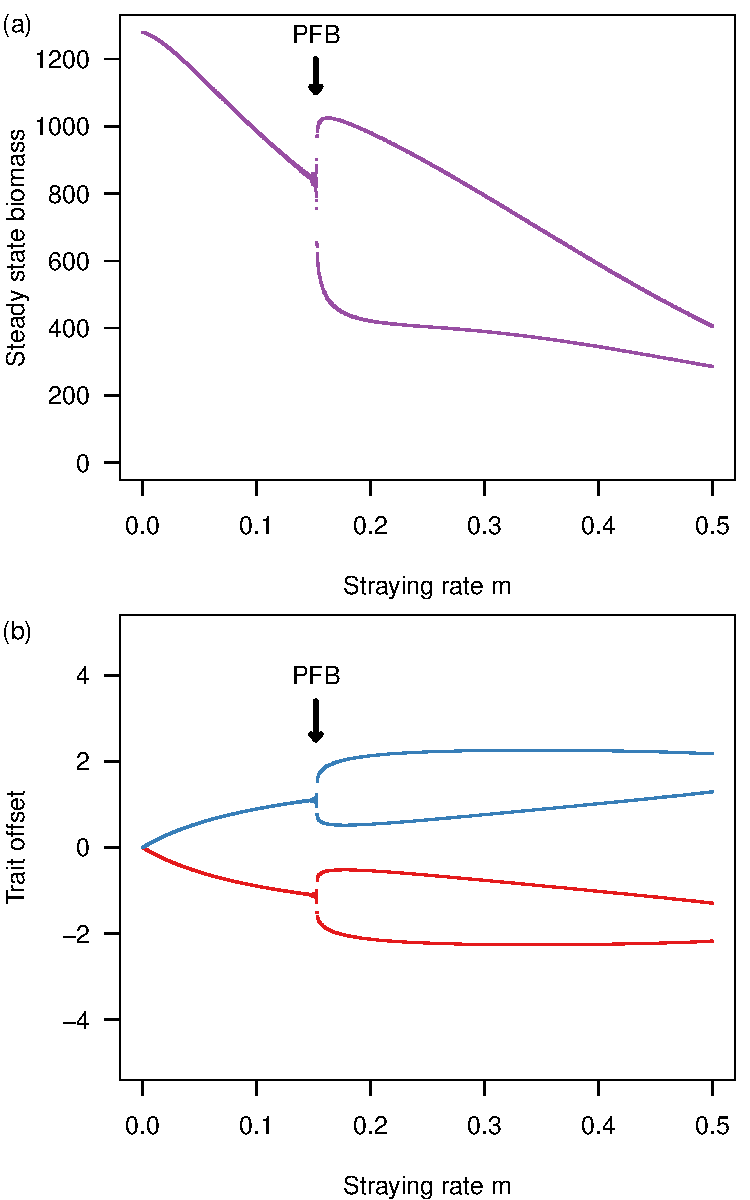
\includegraphics[width=0.4\textwidth]{fig_traj.pdf}
\caption{
(a) The steady-state densities of $N_1$ and $N_2$ vs. the stray rate $m$. Which population attains the low- or high-density state is random due to small applied fluctuations in the initial conditions.
(b) The steady-state trait values measured as the offset from the local optimum $\theta_i - mu_i$, vs. the stray rate $m$. 
DCB marks the discrete cusp bifurcation.
% Unless otherwise indicated, the default parameter values used are: $r_{\rm max}=2$; $Z=0.5$; $\beta=0.001$; $\theta_1=5$; $\Delta\theta=5$; $\tau=1$; $\sigma=1$; $T=1\times10^5$.
} \label{fig:traj}
\end{figure}


\begin{figure*}
  \captionsetup{justification=raggedright,
singlelinecheck=false
}
\centering
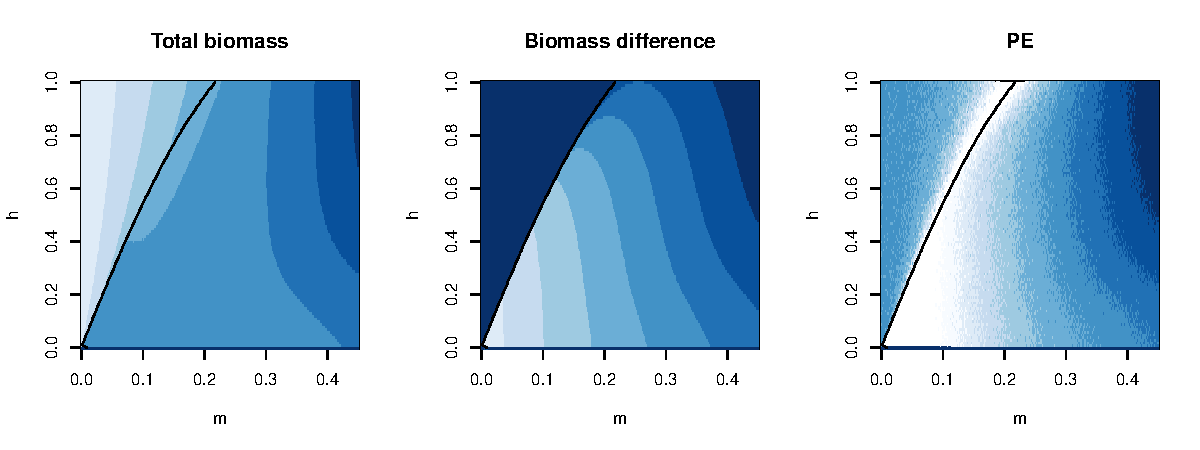
\includegraphics[width=1\textwidth]{fig_MDPE_hm.pdf}
\caption{
(a) Total means $N_t^*$, 
(b) difference in means $\Delta N^*$, and 
(c) the portfolio effect PE as a function of heritability $h^2$ and a constant stray rate $m$. Light colors = high values.
The black line shows the cusp bifurcation separating a single steady-state (left) from alternative stable states (right).
(d) The relationship between the time to recovery following a disturbance and the portfolio effect. Portfolio effects greater than unity corresponds to less synchronization.
} \label{fig:PE}
\end{figure*}


\begin{figure*}
  \captionsetup{justification=raggedright,
singlelinecheck=false
}
\centering
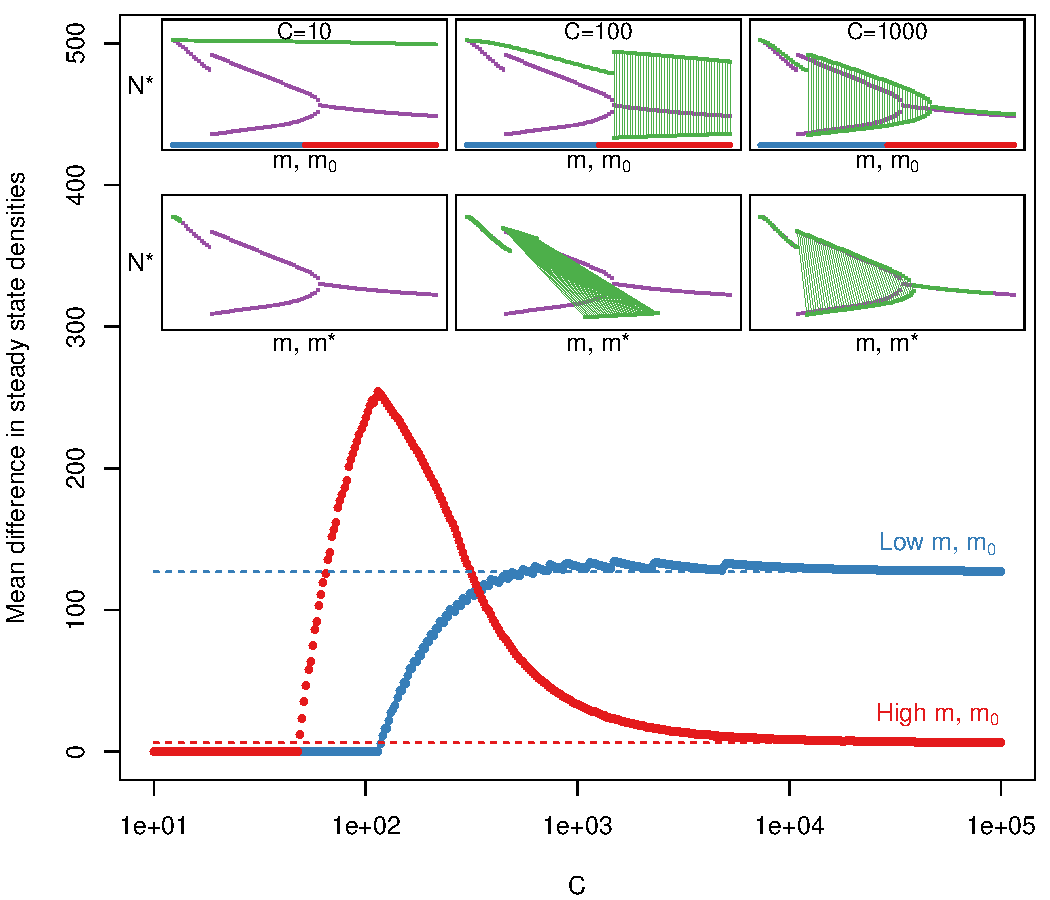
\includegraphics[width=1\textwidth]{fig_meandiff.pdf}
\caption{
Inset: steady states for the constant straying model (purple) and density-dependent straying model (green) for different strengths of collective behavior.
Top row shows steady state densities as a function of individual straying $m_0$; bottom row shows steady state densities as a function of steady state straying $m(t)^*$
Main: Difference in steady states averaged across low straying values ($0 < m,m_0 < 0.25$; blue) and high straying ($0.25 < m,m_0 < 0.5$; red).
} \label{fig:cb}
\end{figure*}


\begin{figure*}
  \captionsetup{justification=raggedright,
singlelinecheck=false
}
\centering
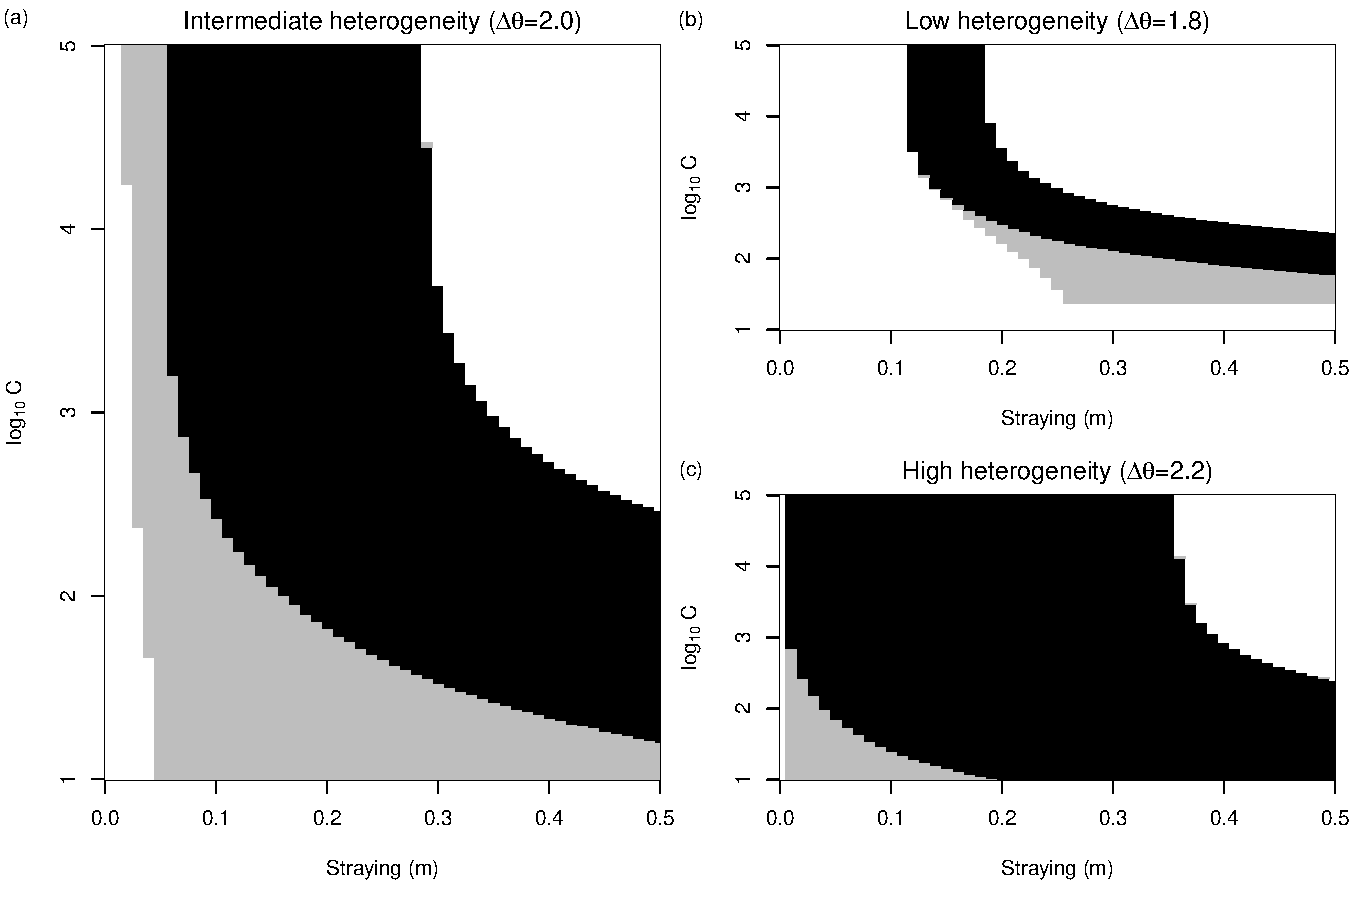
\includegraphics[width=1\textwidth]{fig_hysteresis_ddm.pdf}
\caption{
Regime I (black); Regime II (gray). Leftmost white is symmetric high density stable state regime; white space to left is symmetric low density stable state regime. 
} \label{fig:bifurcationsddm}
\end{figure*}


\begin{figure*}
  \captionsetup{justification=raggedright,
singlelinecheck=false
}
\centering
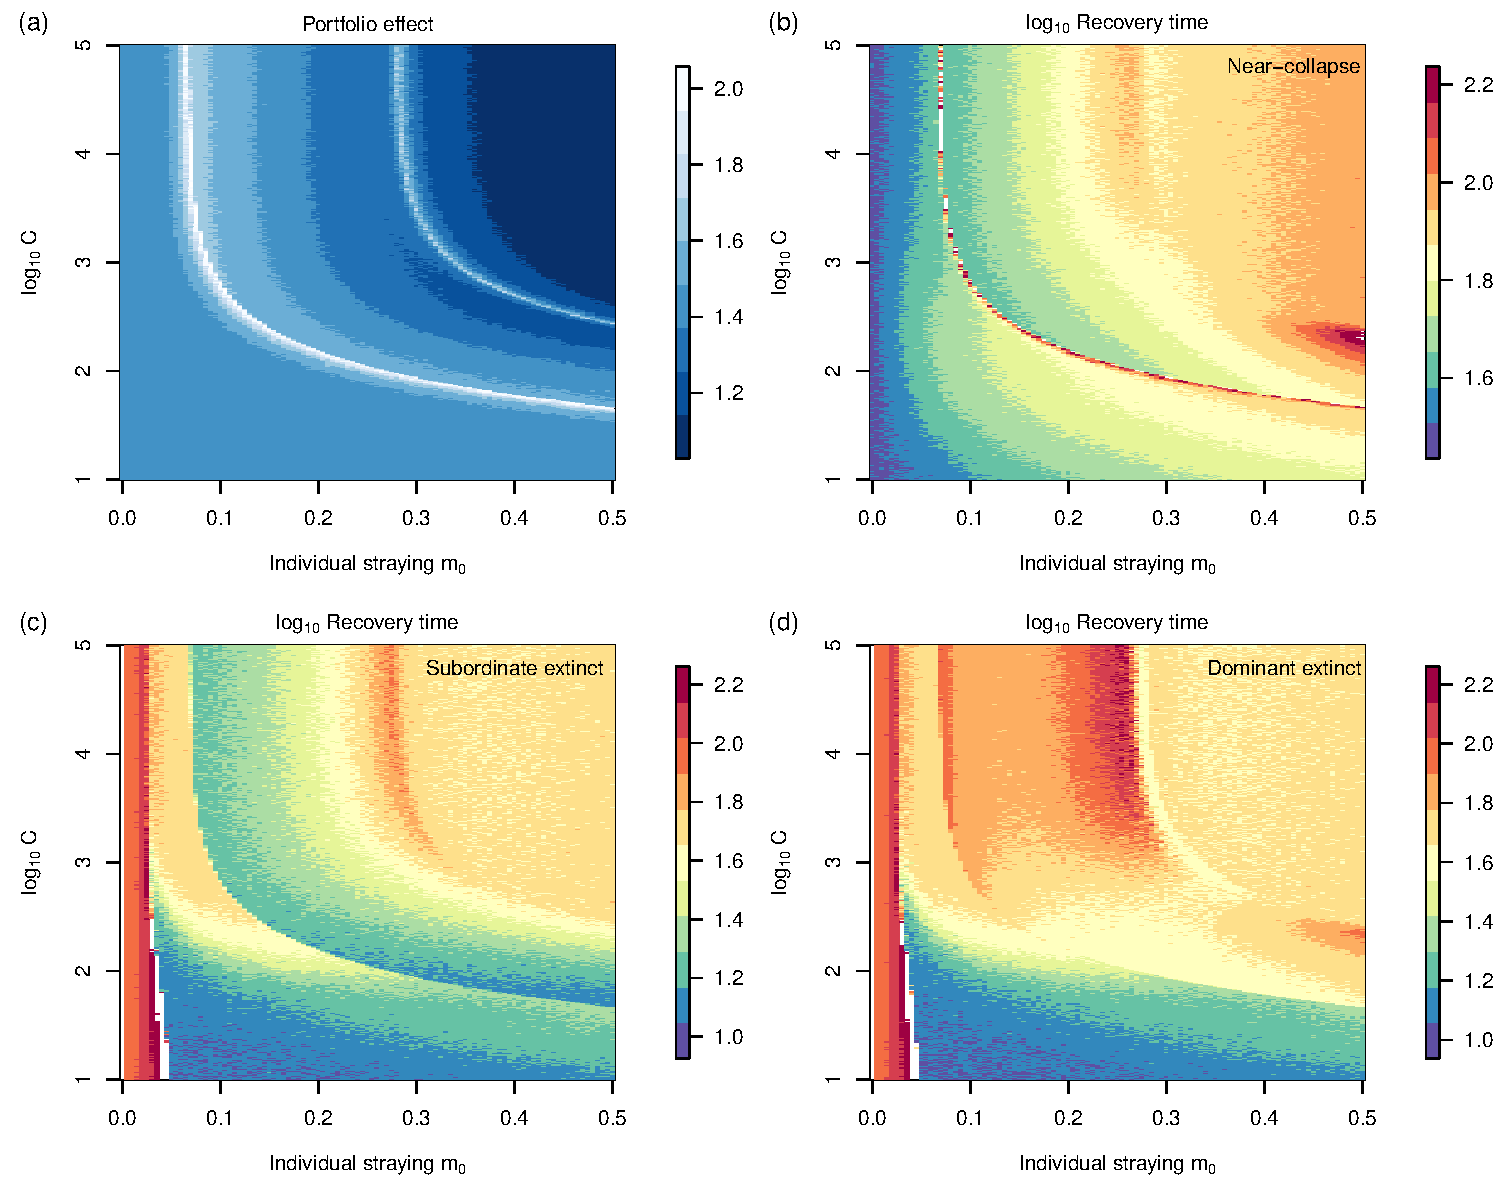
\includegraphics[width=1\textwidth]{fig_rtpe_ddm.pdf}
\caption{
a) Portfolio effect
b) Recovery time following near-collapse of both populations.
} \label{fig:pert}
\end{figure*}


\begin{figure*}
  \captionsetup{justification=raggedright,
singlelinecheck=false
}
\centering
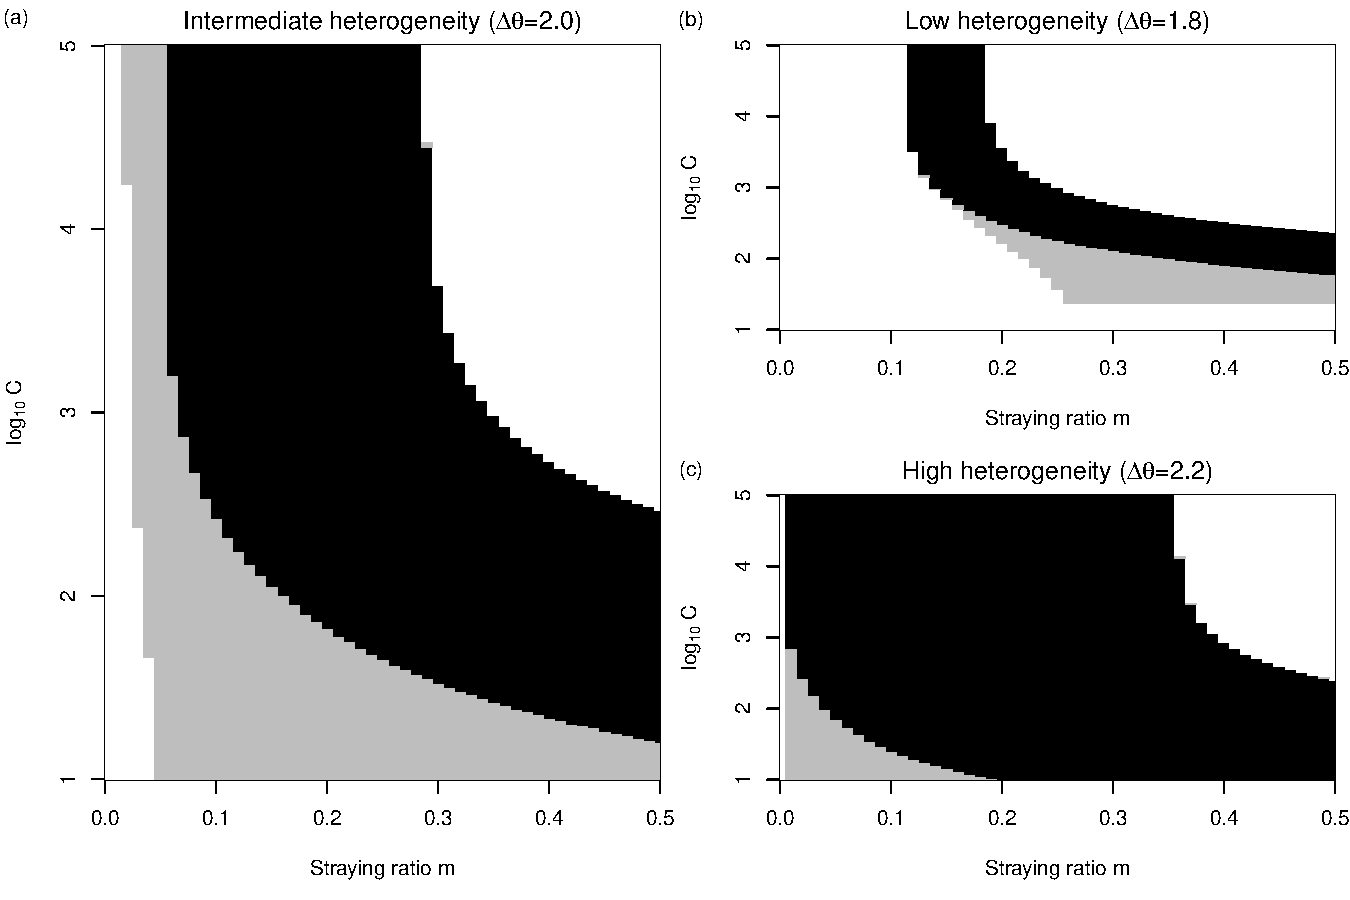
\includegraphics[width=1\textwidth]{fig_hysteresis_ddm_theta.pdf}
\caption{
Each subfig: Regime I (black); Regime II (gray). Leftmost white is symmetric high density stable state regime; white space to left is symmetric low density stable state regime. The cutoff white area on rightmost fig is an artifact.
} \label{fig:hystheta}
\end{figure*}

\begin{figure*}
  \captionsetup{justification=raggedright,
singlelinecheck=false
}
\centering
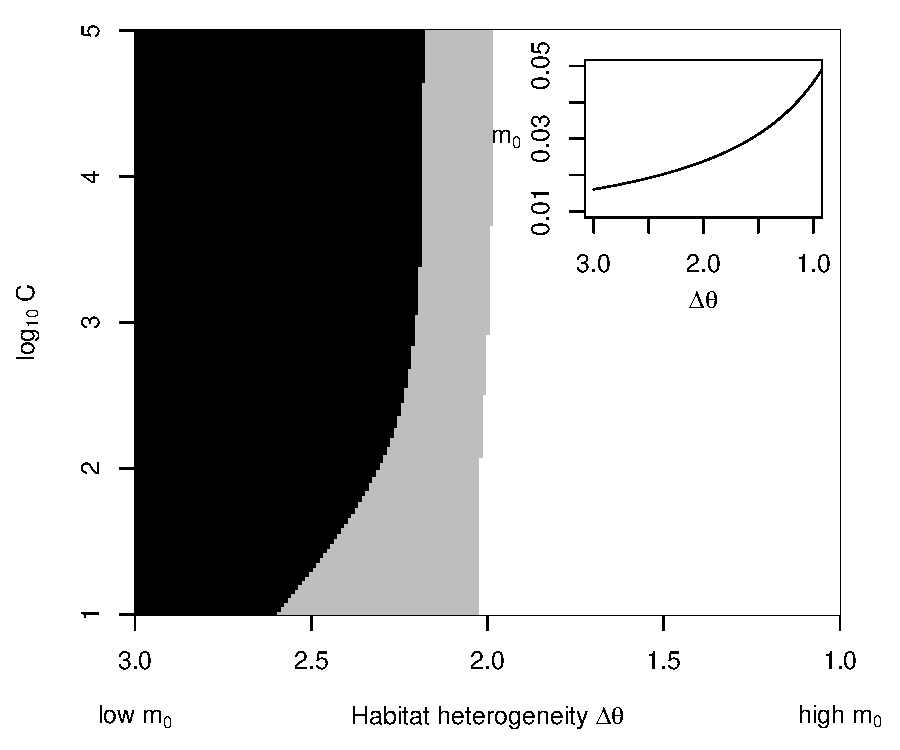
\includegraphics[width=1\textwidth]{fig_hysteresis_ddm_mtheta.pdf}
\caption{
Inset: relationship imposed between $m_0$ and $\Delta\theta$.
Regime I (black); Regime II (gray). Rightmost white is symmetric (low-density) stable state.
} \label{fig:mtheta}
\end{figure*}



% 
% \begin{figure}
%   \captionsetup{justification=raggedright,
% singlelinecheck=false
% }
% \centering
% 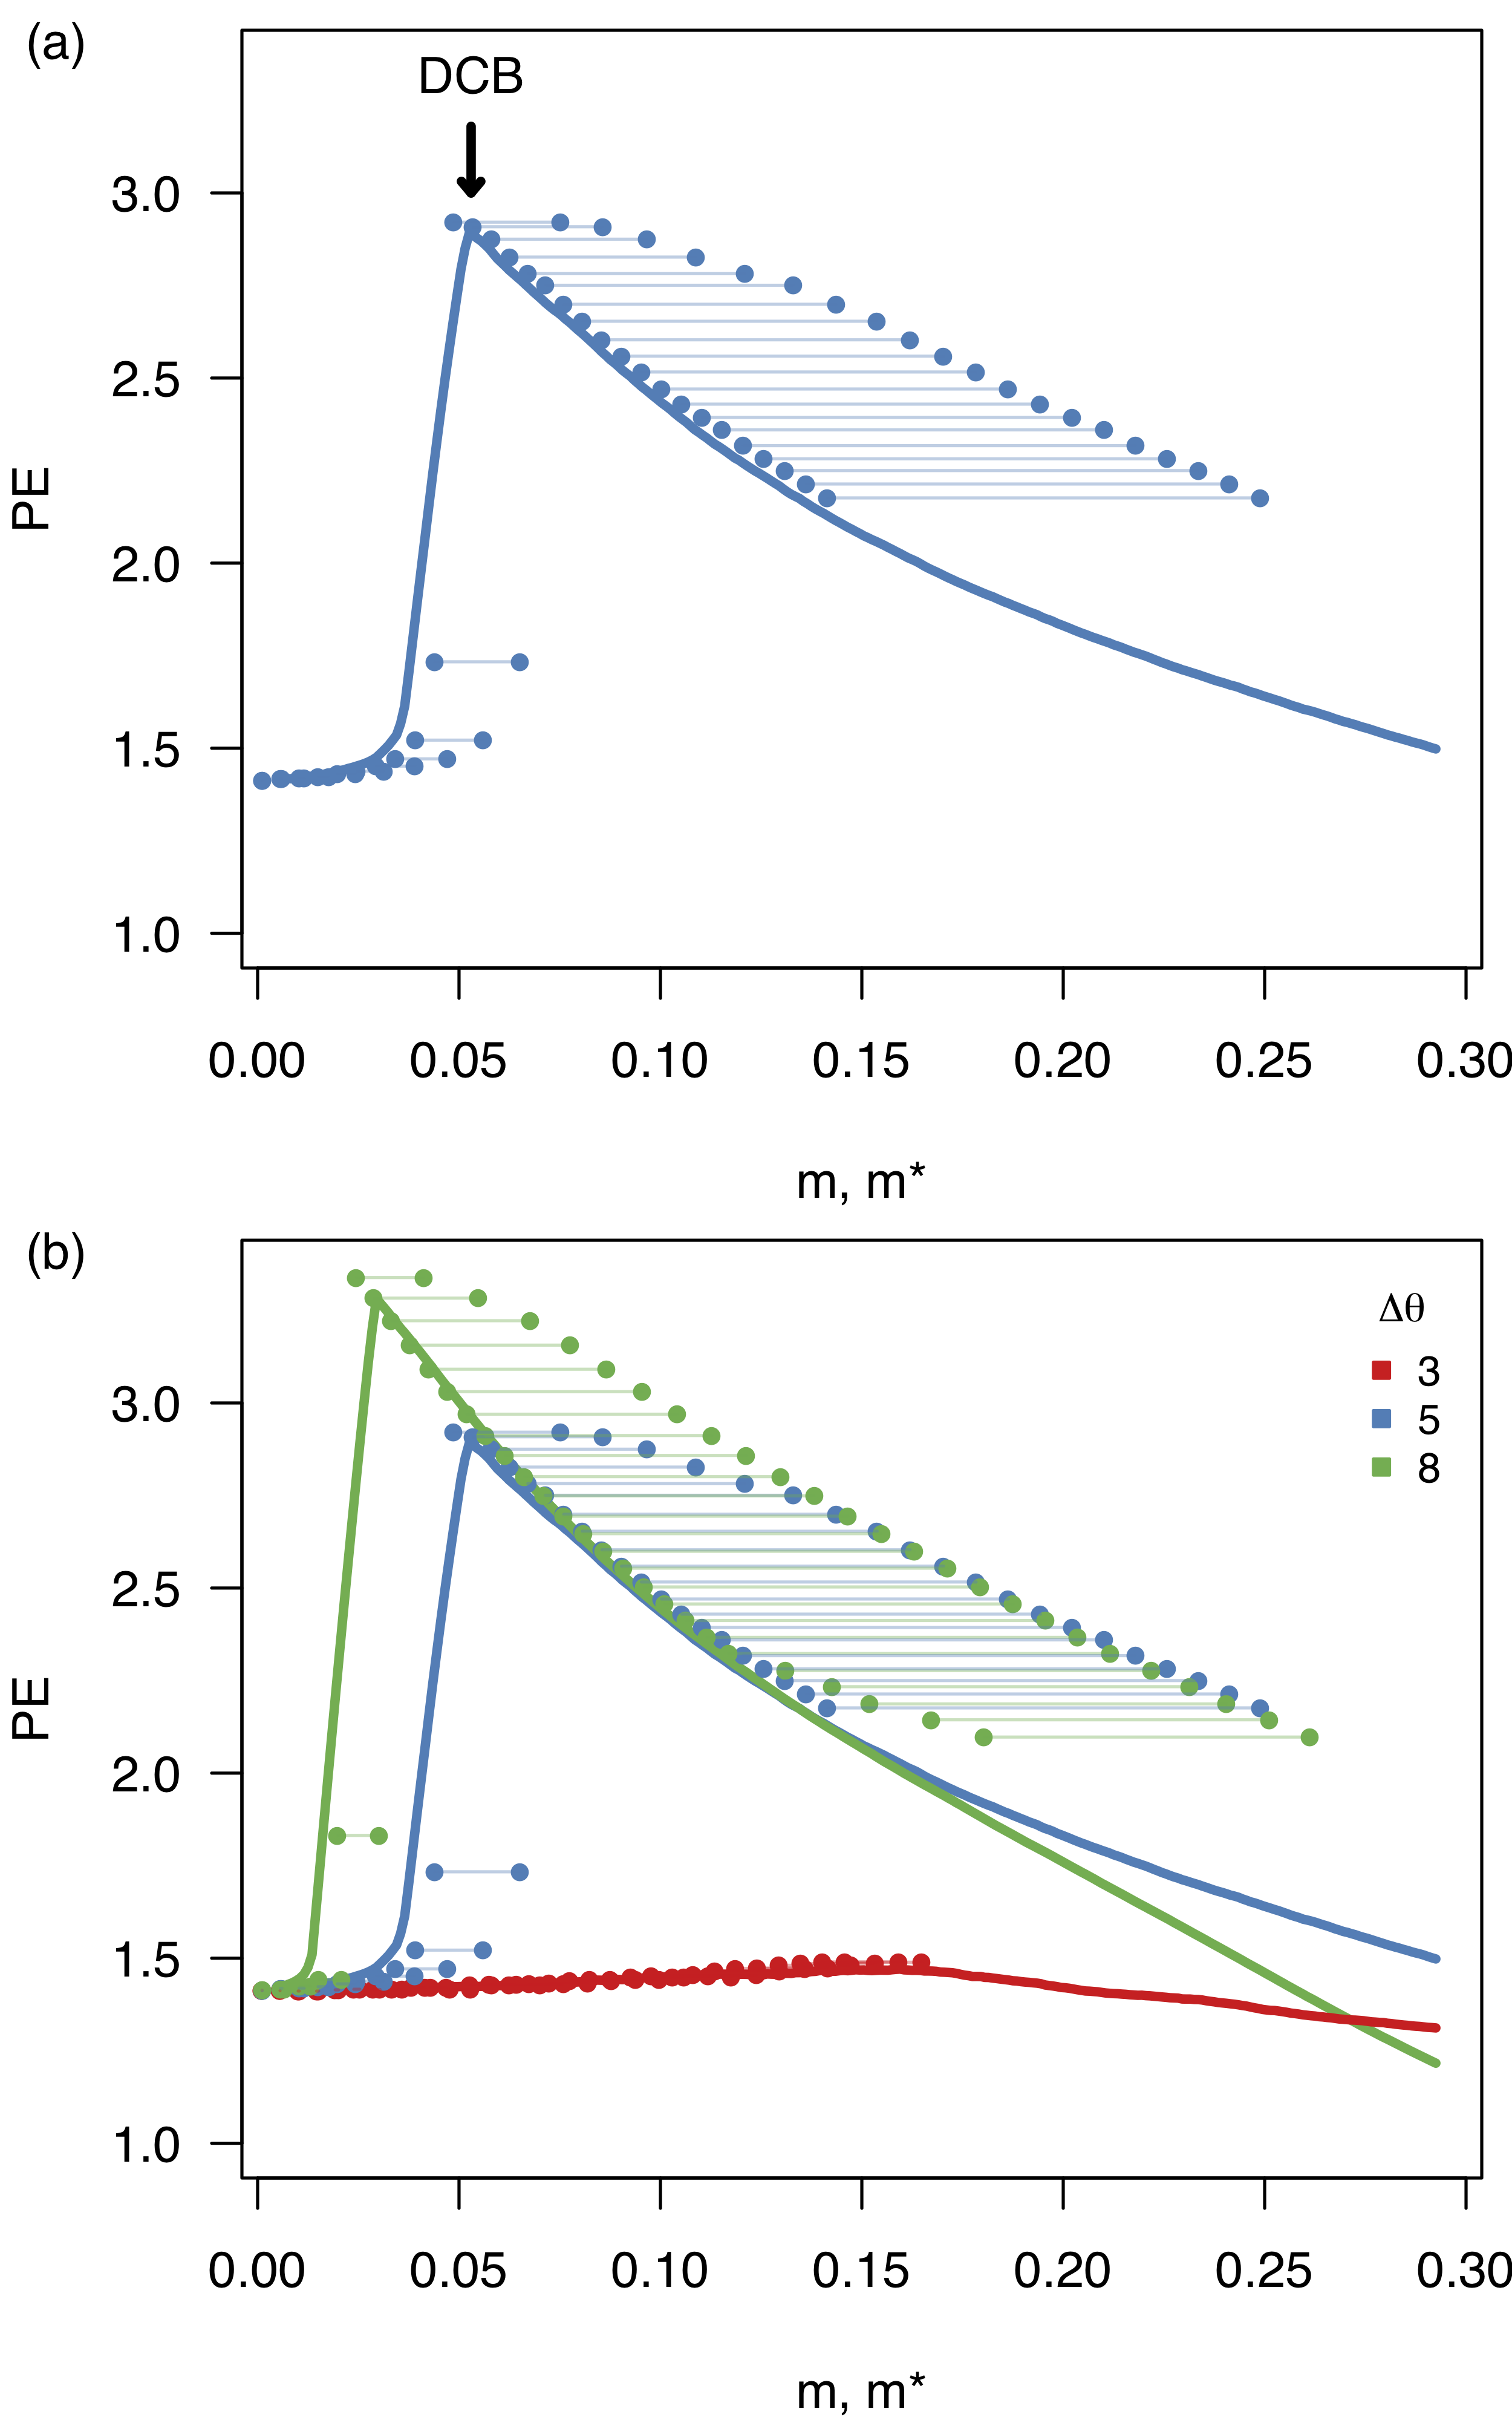
\includegraphics[width=0.4\textwidth]{fig_thetaPEmvm.png}
% \caption{
% (a) Median portfolio effect as a function of a constant stray rate $m$ (solid line) and density-dependent stray rate (point pairs) given heritability is $h^2 < 0.5$ and $\Delta\theta=5$.
% Point pairs connected by a horizontal line represent the PE as a function of density-dependent straying rates, evaluated for both low- and high-density populations at equilibrium. The lower straying rate of a pair is for the larger population; the higher straying rate is for the smaller population.
% (b) Median portfolio effects for habitats with increasing heterogeneity as measured by the difference in regional trait optima $\Delta \theta$ for both constant and density-dependent stray rates as shown in (a).
% Portfolio effects greater than unity corresponds to less synchronization.
% DCB marks the discrete cusp bifurcation.
% } \label{fig:thetaPE}
% \end{figure}
% 
% 
% \begin{figure}
%   \captionsetup{justification=raggedright,
% singlelinecheck=false
% }
%   \centering
%   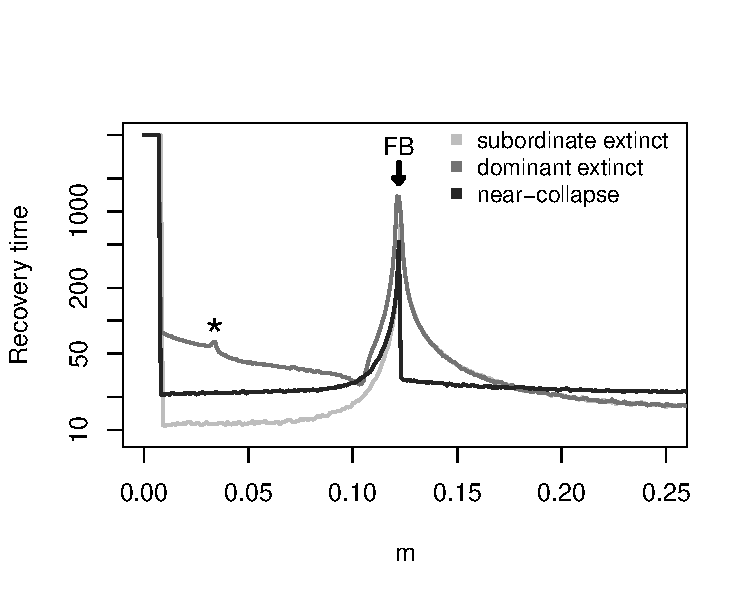
\includegraphics[width=0.5\textwidth]{fig_mtheta_rt.pdf}
%   \caption{
%   Recovery times under three disturbance types for systems where higher habitat heterogeneity $\Delta \theta$ corresponds to lower straying $m$ (see figure \ref{fig:mthetarelation}), and vice versa. 
%   % When straying is distance dependent, $m$ increases as $\Delta\theta$ decreases.
%   The `$*$' marks the value of $m$ below which (low straying between highly heterogeneous environments) there is an inversion between subordinate/dominant states following extinction of the dominant population.
%   DCB marks the discrete cusp bifurcation.
%   } \label{fig:mtheta}
% \end{figure}
% 
% 


%%%%%%%%%%%%%
% SUPPLEMENTARY FIGURES
%%%%%%%%%%%%%

\beginsupplement


\begin{figure}
  \captionsetup{justification=raggedright,
singlelinecheck=false
}
\centering
% 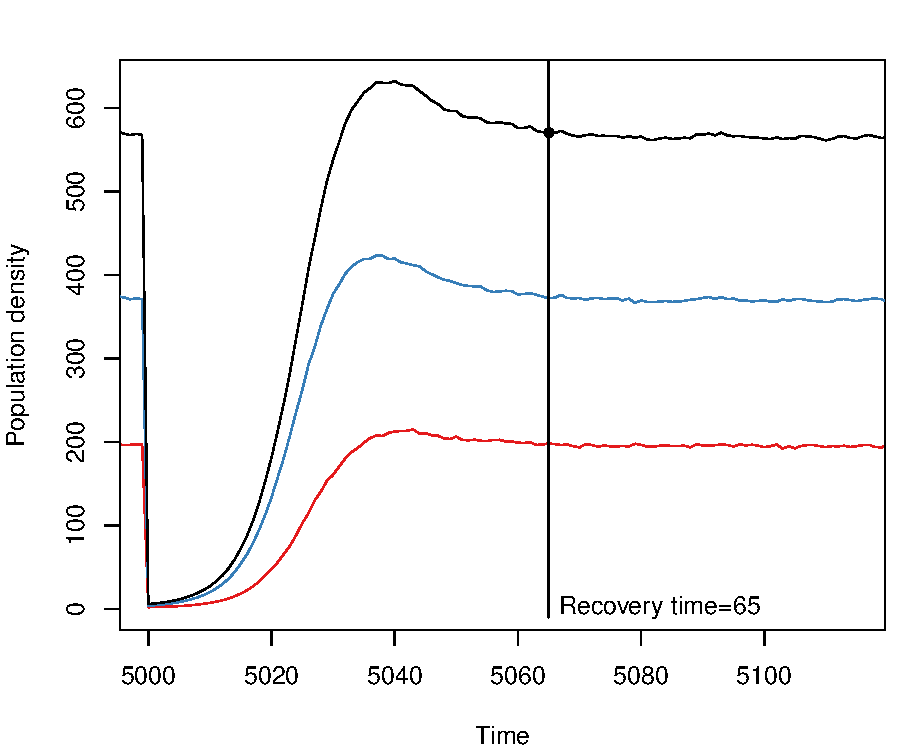
\includegraphics[width=0.35\textwidth]{fig_recovery.pdf}
\caption{
Example of the numerical procedure used to estimate recovery time. After a disturbance is introduced, the recovery time is calculated by measuring the point in time where $N_T$ (in black), which is the aggregate of both populations (blue, red) settles to within one standard deviation of the new equilibrium $N_T^*$. 
} \label{fig:recovery}
\end{figure}

% 
% \begin{figure}
%   \captionsetup{justification=raggedright,
% singlelinecheck=false
% }
% \centering
% 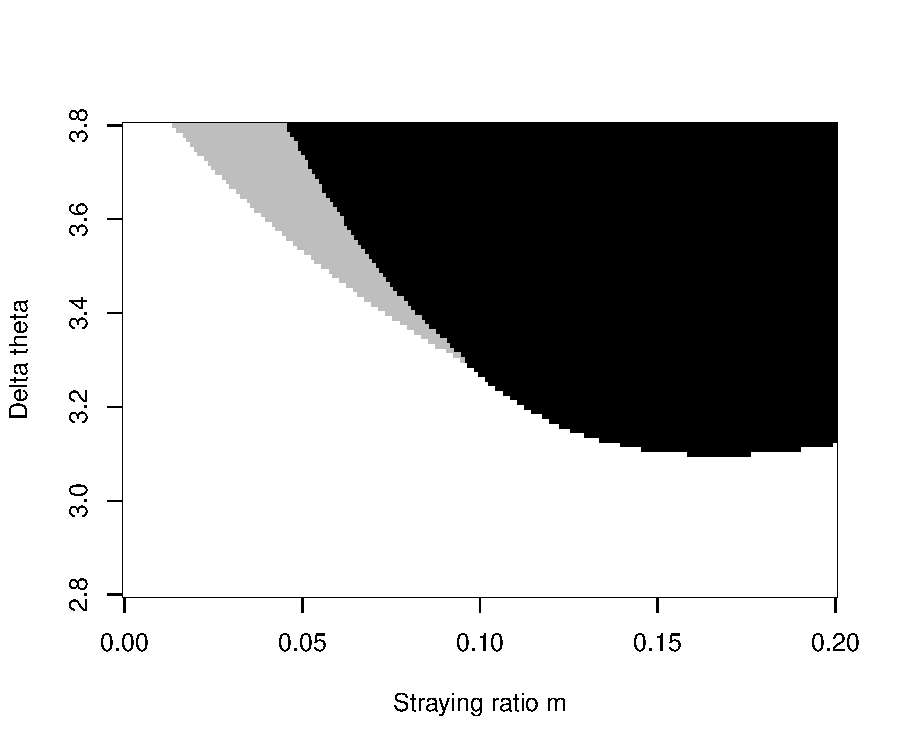
\includegraphics[width=0.35\textwidth]{fig_hysteresis2Dhys.pdf}
% \caption{
% White (low $m$)
% Gray
% Black
% White (high $m$)
% The white/black region is separated by a sub-critical pitchfork bifurcation ($\rm PB_*$); the gray/black region is separated by a super-critical pitchfork bifurcation ($\rm PB^*$); the white/gray region is separated by a fold bifurcation (FB).
% } \label{fig:bifurcations}
% \end{figure}


\begin{figure}
  \captionsetup{justification=raggedright,
singlelinecheck=false
}
\centering
% 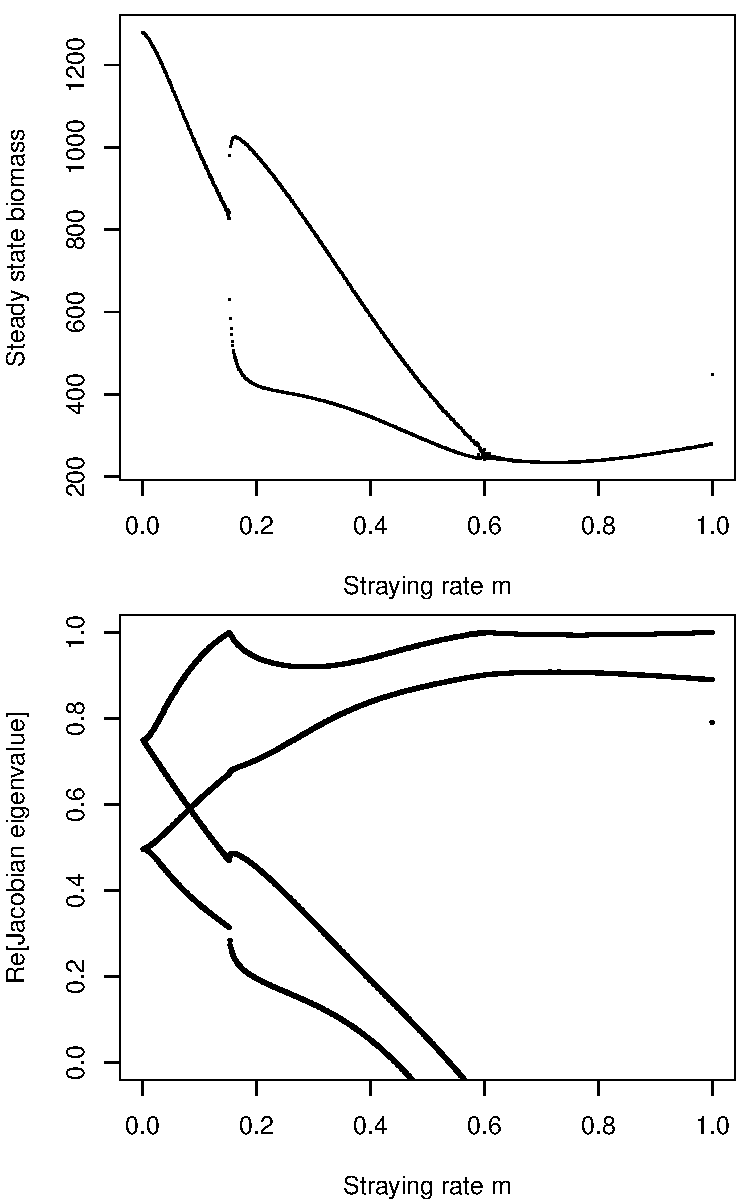
\includegraphics[width=0.35\textwidth]{fig_eigs.pdf}
\caption{
The real parts of the four eigenvalues for the Jacobian matrix of the 4-dimensional system.
The cusp bifurcation occurs when the dominant eigenvalue crosses the unit circle at $+1$. 
} \label{fig:eigs}
\end{figure}



\begin{figure*}
  \captionsetup{justification=raggedright,
singlelinecheck=false
}
\centering
% 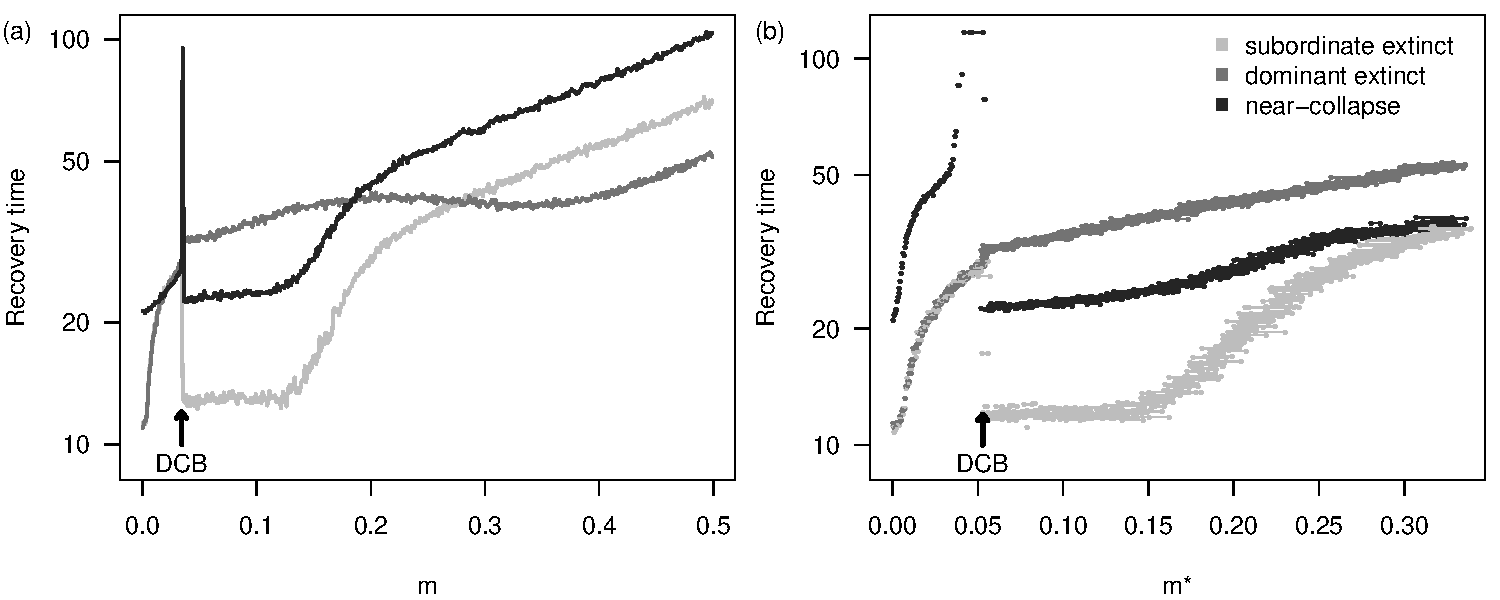
\includegraphics[width=0.9\textwidth]{fig_relax_lowh.pdf}
\caption{
Recovery time of $N_T^*$ following the extinction of either the low-density (light gray) or high-density (gray) population, or the near-collapse of both (dark gray) assuming (a) constant straying rates $m$ and (b) density-dependent straying rates (evaluated at the steady-state $m^*$) with trait heritability $h^2=0.2$.
If $m$ is density-dependent, in the alternative stable state regime there are two straying rates observed: one each for the low- and high-density populations, respectively, which are linked by a horizontal line.
DCB marks the discrete cusp bifurcation.
} \label{fig:relax}
\end{figure*}

\begin{figure*}
  \captionsetup{justification=raggedright,
singlelinecheck=false
}
\centering
% 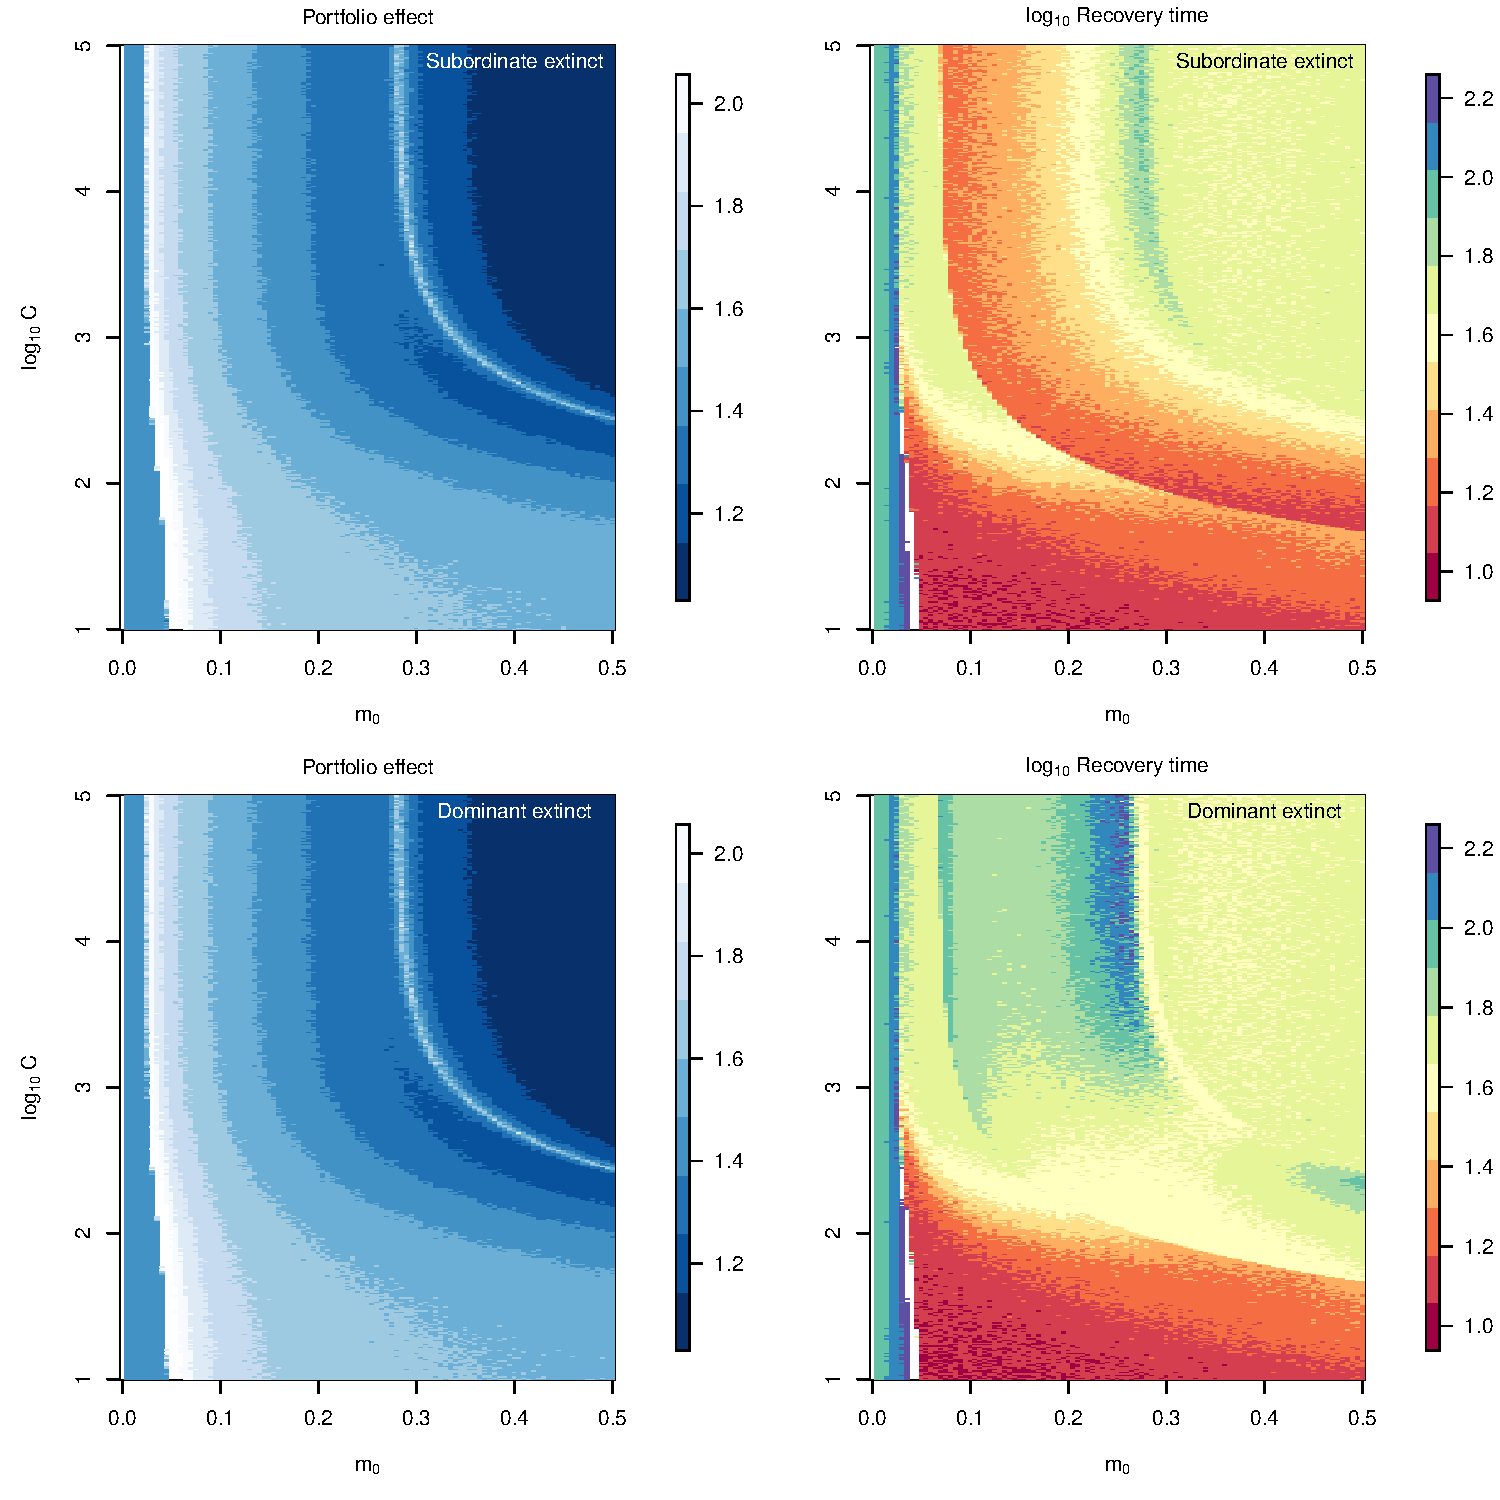
\includegraphics[width=0.9\textwidth]{fig_rtpe_ddmsl.pdf}
\caption{
PE and recovery time after the sole extinction of the subordinate and dominate populations.
} \label{fig:pertlh}
\end{figure*}


\begin{figure}
  \captionsetup{justification=raggedright,
singlelinecheck=false
}
\centering
% 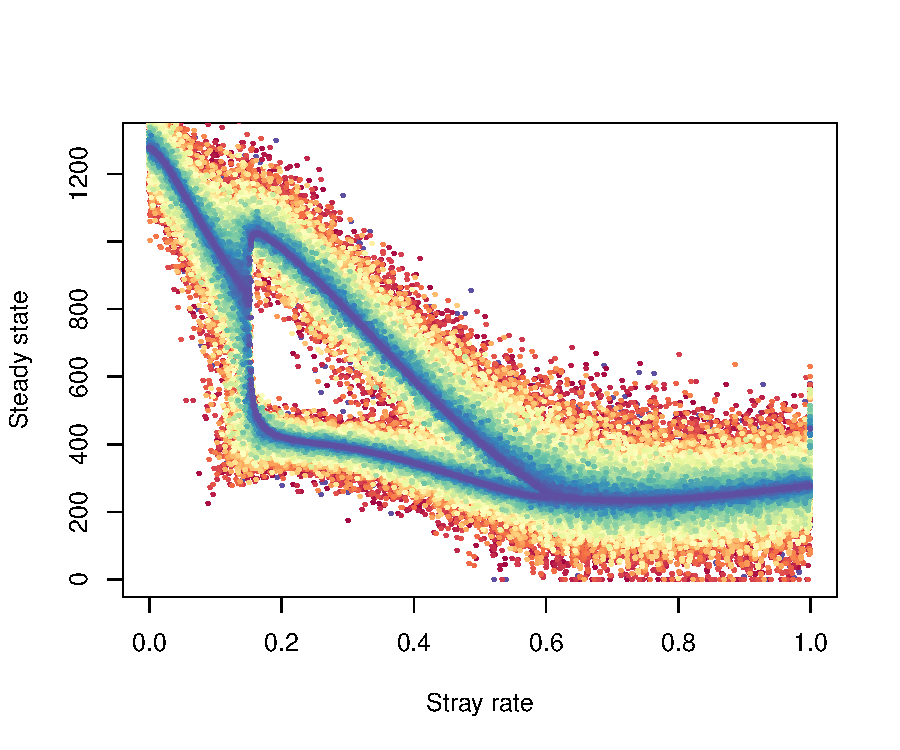
\includegraphics[width=0.35\textwidth]{fig_asymdensity.pdf}
\caption{
Steady-state densities of both populations as a function of $m$, where a cusp bifurcation indicates the emergence of alternative steady-states: one in a dominant state and one in a subordinate state.
Steady-states for populations with symmetrical values ($\alpha=0$) in the vital rates $r_{\rm max}$ and $\beta$ are shown with cool tones.
As the asymmetry among populations between sites increases ($\alpha>0$), their vital rates diverge, such that the maximal growth at sites 1 and 2 is now $r_{\rm max}(1)=r_{\rm max}(1+\tilde{rv}_1)$ and $r_{\rm max}(2)=r_{\rm max}(1+\tilde{rv}_2)$ where $rv_{1,2}$ are independently drawn from $\rm{Normal}(0,\alpha)$ and $r_{\rm max}=2$. 
Similarly the strength of density dependence is calculated at sites 1 and 2 as $\beta(1)=\beta(1+\tilde{rv}_1)$ and $\beta(2)=\beta(1+\tilde{rv}_2)$ where $\tilde{rv}_{1,2}$ are independently drawn from $\rm{Normal}(0,\alpha)$ and $\beta=0.001$.
Steady-states for populations with increasingly asymmetric values ($\alpha\rightarrow 0.1$) for vital rates $r_{\rm max}$ and $\beta$ are shown in warmer tones.
} \label{fig:symmetry}
\end{figure}




\end{document}
